 % The main file for CAMP reports
 % Don't put any content in here.
 % Don't even include content files by using \input or \inlcude.
 % Put your content to TEXT.TEX or include it there using \input.
 % Uses:
 %		SETTINGS.TEX	contains the settings for this document
 %		COMMANDS.TEX	contains commands which can be used while writing
 %		INFO.TEX			contains the author, title and so on for the cover
 %		COVER.TEX			formats the front cover of the document
 %		ABSTRACT.TEX	contains the abstract to be included (if needed)
 %		TEXT.TEX			contains the actual content of the document
 %		BIB.BIB				containt the BibTeX entries for the document


%% Draft document mode
%% Final document
\documentclass[11pt,a4paper,bibtotoc,idxtotoc,headsepline,footsepline,footexclude,BCOR12mm,DIV13]{scrbook}

%\documentclass[11pt,a4paper,bibtotoc,idxtotoc,headsepline,footsepline,footexclude,BCOR20mm,DIV10]{scrbook}

% KOMA-Optionen:
%  bibtotoc: include bibliography in table of contents
%  idxtotoc: include index in table of contents
%  headsepline: use horizontalline under heading
%  BCOR: binding correcion (Bindungskorrektur) (e.g.: BCOR5mm)
%  DIV: Number of sheet sections (used for layout) (e.g.: DIV12)



% include title and author information for the cover
% Set here the title, authors and other stuff to be used for the cover
% This file is used by MAIN.TEX

% set title, authors and stuff for the cover
\def\doctype{Abschlussarbeit in Informatik}
\def\title{Effiziente statistische Methoden f\"ur Datenbanksysteme}
\def\titleGer{Efficient statistical methods for database systems}
\def\author{Thomas Heyenbrock}
\def\date{15.02.2017}

% text to appear in the footer
\def\footertext{}


% include settings
% Included by MAIN.TEX
% Defines the settings for the CAMP report document

\renewcommand{\sectfont}{\normalfont \bfseries}        % Schriftart der Kopfzeile

% manipulate footer
\usepackage{scrpage2}
\pagestyle{scrheadings}
\ifoot[\footertext]{\footertext} % \footertext set in INFO.TEX
%\setkomafont{pagehead}{\normalfont\rmfamily}
\setkomafont{pagenumber}{\normalfont\rmfamily}

%% allow sophisticated control structures
\usepackage{ifthen}

% use Palatino as default font
\usepackage{palatino}

% enable special PostScript fonts
\usepackage{pifont}

% make thumbnails
\usepackage{thumbpdf}

%to use the subfigures
\usepackage{subfigure}


\usepackage{colortbl}


%% show program code\ldots
%\usepackage{verbatim}
%\usepackage{program}

%% enable TUM symbols on title page
\usepackage{styles/tumlogo}


\usepackage{multirow}

%% use colors
\usepackage{color}

%% make fancy math
\usepackage{amsmath}
\usepackage{amsfonts}
\usepackage{amssymb}
\usepackage{textcomp}
\usepackage{yhmath} % f�r die adots
%% mark text as preliminary
%\usepackage[draft,german,scrtime]{prelim2e}

%% create an index
\usepackage{makeidx}

% for the program environment
\usepackage{float}

%% load german babel package for german abstract
%\usepackage[german,american]{babel}
\usepackage[german,english]{babel}
\selectlanguage{german}

% use german characters as well
% \usepackage[latin1]{inputenc}       % allow Latin1 characters
\usepackage[utf8]{inputenc}       % allow UTF8 characters

% use initals dropped caps - doesn't work with PDF
\usepackage{dropping}

%% use code formatting
\usepackage[T1]{fontenc}
\usepackage{lmodern}
\usepackage{minted}

\usepackage{styles/shortoverview}

\usepackage{caption}
\captionsetup[table]{name=Tabelle}

\usepackage{qtree}

%----------------------------------------------------
%      Graphics and Hyperlinks
%----------------------------------------------------

%% check for pdfTeX
\ifx\pdftexversion\undefined
 %% use PostScript graphics
 \usepackage[dvips]{graphicx}
 \DeclareGraphicsExtensions{.eps,.epsi}
 \graphicspath{{figures/}{figures/review}}
 %% allow rotations
 \usepackage{rotating}
 %% mark pages as draft copies
 %\usepackage[english,all,light]{draftcopy}
 %% use hypertex version of hyperref
 \usepackage[hypertex,hyperindex=false,colorlinks=false]{hyperref}
\else %% reduce output size \pdfcompresslevel=9
 %% declare pdfinfo
 %\pdfinfo {
 %  /Title (my title)
 %  /Creator (pdfLaTeX)
 %  /Author (my name)
 %  /Subject (my subject	)
 %  /Keywords (my keywords)
 %}
 %% use pdf or jpg graphics
 \usepackage[pdftex]{graphicx}
 \DeclareGraphicsExtensions{.jpg,.JPG,.png,.pdf,.eps}
 \graphicspath{{figures/}}

 %% Load float package, for enabling floating extensions
 \usepackage{float}

 %% allow rotations
 \usepackage{rotating}
 %% use pdftex version of hyperref
 \usepackage[pdftex,colorlinks=true,linkcolor=red,citecolor=red,%
 anchorcolor=red,urlcolor=red,bookmarks=true,%
 bookmarksopen=true,bookmarksopenlevel=0,plainpages=false%
 bookmarksnumbered=true,hyperindex=false,pdfstartview=%
 ]{hyperref}
%
%\usepackage[pdftex,colorlinks=false,linkcolor=red,citecolor=red,%
% anchorcolor=red,urlcolor=red,bookmarks=true,%
% bookmarksopen=true,bookmarksopenlevel=0,plainpages=false%
% bookmarksnumbered=true,hyperindex=false,pdfstartview=%
% ]{hyperref}
\fi




%% Fancy chapters
%\usepackage[Lenny]{fncychap}
%\usepackage[Glenn]{fncychap}
%\usepackage[Bjarne]{fncychap}

%\usepackage[avantgarde]{quotchap}

% set the bibliography style
%\bibliographystyle{styles/bauermaNum}
%\bibliographystyle{alpha}
\bibliographystyle{plain}


% include commands
% Commands to be used within the TUM report document
% Included by MAIN.TEX
% Please include your own cool commands here. 
% Be only sure to comment it sufficiently so others can use it.

%-------------------------------------------------------------
%                      Own Commands
%-------------------------------------------------------------


%-------------------------------------------------------------
% math stuff -------------------------------------------------

% nice R, N, C
\newcommand{\nat}{\mathbb{N}}
\newcommand{\real}{\mathbb{R}}
\newcommand{\compl}{\mathbb{C}}



% norm
\newcommand{\norm}[1]{\left\| #1 \right\|}

% un demi
\newcommand{\half}{\frac{1}{2}}

% parantheses
\newcommand{\parenth}[1]{ \left( #1 \right) }
\newcommand{\bracket}[1]{ \left[ #1 \right] }
\newcommand{\accolade}[1]{ \left\{ #1 \right\} }
%\newcommand{\angle}[1]{ \left\langle  #1 \right\rangle }

% partial derivative: %#1 function, #2 which variable
% simple / single line version
\newcommand{\pardevS}[2]{ \delta_{#1} f(#2) }
% fraction version
\newcommand{\pardevF}[2]{ \frac{\partial #1}{\partial #2} }

% render vectors: 3 and 4 dimensional
\newcommand{\veciii}[3]{\left[ \begin{array}[h]{c} #1 \\ #2 \\ #3	\end{array} \right]}
\newcommand{\veciv}[4]{\left[ \begin{array}[h]{c} #1 \\ #2 \\ #3 \\ #4	\end{array} \right]}

% render matrices: 3  dimensional (arguments in row first order)
\newcommand{\matiii}[9]{\left[ \begin{array}[h]{ccc} #1 & #2 & #3 \\ #4 & #5 & #6 \\ #7 & #8 & #9	\end{array} \right]}
%DOESN'T WORK,DON'T KNOW WHY \newcommand{\mativ}[16]{\left[ \begin{array}[h]{cccc} #1 & #2 & #3 & #4 \\ #5 & #6 & #7 & #8 \\ #9 & #10 & #11 & #12 \\ #13 & #14 & #15 & #16 \end{array} \right]}


%-------------------------------------------------------------
%-------------------------------------------------------------


%-------------------------------------------------------------
% some abreviations ------------------------------------------
\newcommand{\Reg}{$^{\textregistered}$}
\newcommand{\reg}{$^{\textregistered}$ }
\newcommand{\Tm}{\texttrademark}
\newcommand{\tm}{\texttrademark~}
\newcommand {\bsl} {$\backslash$}

%-------------------------------------------------------------
%-------------------------------------------------------------


%-------------------------------------------------------------
% formating --------------------------------------------------

% Theorem & Co environments and counters
\newtheorem{theorem}{Theorem}[chapter]
\newtheorem{lemma}[theorem]{Lemma}
\newtheorem{corollary}[theorem]{Corollary}
\newtheorem{remark}[theorem]{Remark}
\newtheorem{definition}[theorem]{Definition}
\newtheorem{equat}[theorem]{Equation}
\newtheorem{example}[theorem]{Example}
\newtheorem{algorithm}[theorem]{Algorithm}

% inserting figures
\newcommand{\insertfigure}[4]{ % Filename, Caption, Label, Width percent of textwidth
	\begin{figure}[htbp]
		\begin{center}
			\includegraphics[width=#4\textwidth]{#1}
		\end{center}
		\vspace{-0.4cm}
		\caption{#2}
		\label{#3}
	\end{figure}
}




% referecing figures

\newcommand{\refFigure}[1]{ %label
	figure \ref{#1}
}
\newcommand{\refChapter}[1]{ %label
	chapter \ref{#1}
}

\newcommand{\refSection}[1]{ %label
	section \ref{#1}
}

\newcommand{\refParagraph}[1]{ %label
	paragraph \ref{#1}
}

\newcommand{\refEquation}[1]{ %label
	equation \ref{#1}
}

\newcommand{\refTable}[1]{ %label
	table \ref{#1}
}




\newcommand{\rigidTransform}[2]
{
	${}^{#2}\!\mathbf{H}_{#1}$
}

%code, in typewriter
\newcommand{\code}[1]
 {\texttt{#1}}

% comment that appears on the border - very practical !!!
\newcommand{\comment}[1]{\marginpar{\raggedright \noindent \footnotesize {\sl #1} }}

% page clearing
\newcommand{\clearemptydoublepage}{%
  \ifthenelse{\boolean{@twoside}}{\newpage{\pagestyle{empty}\cleardoublepage}}%
  {\clearpage}}


%-------------------------------------------------------------
%-------------------------------------------------------------


\newcommand{\etAl}{\emph{et al.}\mbox{ }}


%\makeindex
	%% inter line spacing
%\linespread{1.0}

\makeglossary

\begin{document}

	\frontmatter


	% The front cover for the TUM report document.
% Included by MAIN.TEX


%--------------------------------------------------
% The Front Cover
%--------------------------------------------------

% The front cover for the TUM document.
% Included by MAIN.TEX


%--------------------------------------------------
% The Front Cover
%--------------------------------------------------

% correct BCOR - undo at the end !!!
\def\bcorcor{0.15cm}
\addtolength{\hoffset}{\bcorcor}

\thispagestyle{empty}

 \vspace{4cm}
\begin{center}
	       \oTUM{4cm}
	   
	   \vspace{5mm}     
	   \huge FAKULT{\"A}T F{\"U}R INFORMATIK\\ 
	   \vspace{0.5cm}
	 \large DER TECHNISCHEN UNIVERSIT{\"A}T M{\"U}NCHEN\\
    \vspace{1mm}
        
	\end{center}
		

\vspace{15mm}
\begin{center}

   {\Large \doctype}

  \vspace{20mm}
  
  {\huge\bf \title}\\%[3ex]
  
  
  \vspace{15mm}
  
  
  {\LARGE  \author}
  
  \vspace{10mm}
  
  \begin{figure}[h!]
  \centering
   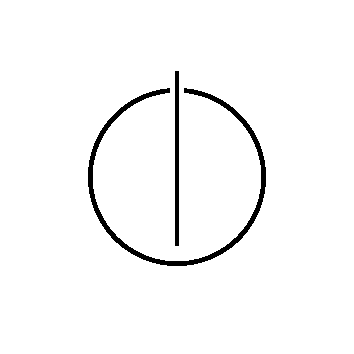
\includegraphics[width=4cm]{styles/informat.png}
  \end{figure}
  
  \end{center}
%	\clearemptydoublepage
%
%	% The titlepage for the CAMP report document.
% Included by MAIN.TEX


%--------------------------------------------------
% The title page
%--------------------------------------------------

% correct BCOR - undo at the end !!!
\def\bcorcor{0.15cm}
\addtolength{\hoffset}{\bcorcor}

\thispagestyle{empty}

 \vspace{10mm}
\begin{center}
	       \oTUM{4cm}

	   \vspace{5mm}
	   \huge FAKULT{\"A}T F{\"U}R INFORMATIK\\
	   \vspace{0.5cm}
	 \large DER TECHNISCHEN UNIVERSIT{\"A}T M{\"U}NCHEN\\

	\end{center}


\vspace{10mm}
\begin{center}

   {\Large \doctype}

  \vspace{10mm}

  {\LARGE \title}\\


  \vspace{10mm}


  {\LARGE  \titleGer}\\


  \vspace{10mm}

    %\hfill
    \begin{tabular}{ll}
	   \Large Autor:     & \Large \author \\[2mm]
	   \Large Supervisor:    & \Large Prof. Alfons Kemper \\[2mm]
	   \Large Advisor:	& \Large Maximilian E. Schüle, M.Sc. \\[2mm]
	   \Large Datum:       & \Large \date
	 \end{tabular}

	 \vspace{5mm}

	 \begin{figure}[h!]
  \centering
   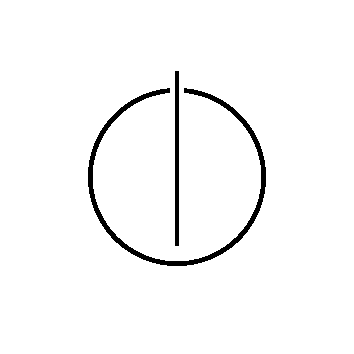
\includegraphics[width=4cm]{styles/informat.png}
  \end{figure}


\end{center}

% undo BCOR correction
\addtolength{\hoffset}{\bcorcor}



%	\input{components/cover_maschmeyer}
	\clearemptydoublepage

	% The titlepage for the CAMP report document.
% Included by MAIN.TEX


%--------------------------------------------------
% The title page
%--------------------------------------------------

% correct BCOR - undo at the end !!!
\def\bcorcor{0.15cm}
\addtolength{\hoffset}{\bcorcor}

\thispagestyle{empty}

 \vspace{10mm}
\begin{center}
	       \oTUM{4cm}

	   \vspace{5mm}
	   \huge FAKULT{\"A}T F{\"U}R INFORMATIK\\
	   \vspace{0.5cm}
	 \large DER TECHNISCHEN UNIVERSIT{\"A}T M{\"U}NCHEN\\

	\end{center}


\vspace{10mm}
\begin{center}

   {\Large \doctype}

  \vspace{10mm}

  {\LARGE \title}\\


  \vspace{10mm}


  {\LARGE  \titleGer}\\


  \vspace{10mm}

    %\hfill
    \begin{tabular}{ll}
	   \Large Autor:     & \Large \author \\[2mm]
	   \Large Supervisor:    & \Large Prof. Alfons Kemper \\[2mm]
	   \Large Advisor:	& \Large Maximilian E. Schüle, M.Sc. \\[2mm]
	   \Large Datum:       & \Large \date
	 \end{tabular}

	 \vspace{5mm}

	 \begin{figure}[h!]
  \centering
   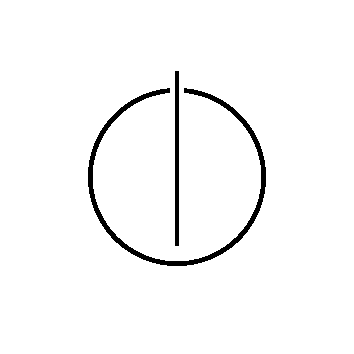
\includegraphics[width=4cm]{styles/informat.png}
  \end{figure}


\end{center}

% undo BCOR correction
\addtolength{\hoffset}{\bcorcor}



	\clearemptydoublepage


\thispagestyle{empty}
\selectlanguage{german}
	\vspace*{0.8\textheight}
	\noindent
	Ich versichere, dass ich diese Abschlussarbeit selbständig verfasst und nur
	die angegebenen Quellen und Hilfsmittel verwendet habe.

	\vspace{15mm}
	\noindent
	München, den \today \hspace{5cm} \author
\selectlanguage{english}
\newpage


	% \clearemptydoublepage
\phantomsection
\addcontentsline{toc}{chapter}{Acknowledgements}	


%\chapter*{Acknowledgements}

\vspace*{2cm}

\begin{center}
{\Large \bf Acknowledgments}
\end{center}

\vspace{1cm}




If someone contributed to the thesis... might be good to thank them here.

	% Abstract for the TUM report document
% Included by MAIN.TEX


\clearemptydoublepage
\phantomsection
\addcontentsline{toc}{chapter}{Zusammenfassung}





\vspace*{2cm}
\begin{center}
{\Large \bf Zusammenfassung}
\end{center}
\vspace{1cm}

Das Ziel der vorliegenden Arbeit ist es, die Durchführung von statistischen Methoden in relationalen Datenbanksystemen zu demonstrieren. Das statistische Konzept, dass dazu verwendet wird, ist die lineare und die logistische Regressionsanalyse. Dazu werden zuerst kurz die mathematischen Grundlagen erklärt. Danach wird die Umsetzung der Regressionsanalyse mit verschiedenen Programmiersprachen demonstriert, insbesondere in zwei relationalen Datenbanken. Zum Abschluss werden die Implementierungen verglichen und ein mögliches Erweiterungspotenzial für relationale Datenbanksysteme wird erläutert.

\vspace*{3cm}
\begin{center}
{\Large \bf Abstract}
\end{center}
\vspace{1cm}

The goal of this thesis is to demonstrate the implementation of statistical methods in relational database systems. The statistical concepts used are linear and logistic regression analysis. First, the mathematical basics are explained briefly. Then the implementation of the regression analysis will be demonstrated with different programming languages, especially in two relational databases. Finally, the implementations are compared and an expansion potential for relational database systems is explained.


	\renewcommand{\contentsname}{Inhaltsverzeichnis}
	\tableofcontents

	\mainmatter

	% Included by MAIN.TEX
% Put your content in here or include it by using \input (\include won't work)

\addtolength{\evensidemargin}{-12mm}

\chapter{Einführung und typische statistische Problemstellungen}
\label{chapter:1}

Die Statistik ist ein Teilgebiet der Mathematik, in welchem Methoden zum Umgang und zur Verarbeitung von Daten behandelt werden. Dabei wird oft ein vorhandener Satz an Daten, auch Stichprobe genannt, betrachtet und analysiert, um daraus Vorhersagen für die Gesamtheit aller Daten zu treffen. Den Teilbereich der Statistik, welcher sich mit solchen Problemen befasst, nennt man induktive oder schließende Statistik.

Betrachtet man beispielsweise die Körpergröße und das Gewicht von 100 Testpersonen, dann kann man sich fragen, ob diese beiden Merkmale in Zusammenhang stehen. Insbesondere ist interessant, wie man einen möglichen Zusammenhang quantitativ darstellen kann und ob man neben der Körpergröße auch andere Faktoren für das Gewicht einer Person betrachten sollte. Das sind beispielhafte Typen von Fragen, welchen man in der Statistik oft begegnet.

Die Statistik zeigt Methoden und Vorgehensweisen auf, wie man solche Fragen angehen und beantworten kann. Ein oft verwendetes Verfahren ist die Regression bzw. die Regressionsanalyse. Hier sucht und analysiert man Beziehungen zwischen mehreren Variablen und versucht diese quantitativ zu beschreiben.

Greifen wir das obige Beispiel wieder auf: Bei der Regression sucht man nach einer Formel, welche für gegebene Körpergröße das Gewicht einer Person möglichst gut schätzt. Oft trifft man Annahmen über die Art der Beziehung zwischen den Dimensionen, um die Suche a priori einzugrenzen. Man beschränkt sich in vielen Fällen auf lineare Funktionen, da solche leicht zu behandeln sind. In der Praxis sind aber auch allgemeine Potenzfunktionen, exponentielle Funktionen oder logistische Funktionen bzw. Beziehungen oft anzutreffen.

Es gibt speziell für Statistik entwickelte Software, seien es einfache Programmiersprachen wie das R-Projekt oder komplexere Programme mit grafischem Interface wie SPSS von IBM. Die Daten, welche man als Basis für Analysen verwendet, müssen aber an einer anderen Stelle gespeichert und verwaltet werden. Oft liegen diese in einer Datenbank und müssen zuerst in das Analysetool importiert werden.

Konzeptuell ist eine Datenbank nicht für Regressionsanalyse geschaffen. Dennoch ist es in relationalen Datenbanksystemen mit SQL möglich, Regression direkt in der Datenbank durchzuführen. Damit übergeht man den eben genannten Schritt des Importierens. Man kann außerdem die Ergebnisse der Analyse direkt aus der Datenbank abfragen oder dort weiterverwenden.

Diese Arbeit wird zuerst das Konzept der Regression konkreter einführen und die mathematischen Grundlagen darlegen. Darauf aufbauend betrachten wir Implementierungen für Regressionsanalyse in verschiedenen Programmiersprachen. Hier soll insbesondere die Anwendung von Regressionsanalyse mit Hilfe von SQL demonstriert werden. Danach wollen wir die Sprachen bezüglich der Laufzeit miteinander vergleichen und noch kurz auf das Erweiterungspotenzial für relationale Datenbanksysteme eingehen.


\chapter{Grundlagen statistischer Methoden}
\label{chapter:2}

Bei der Regressionsanalyse geht es im Allgemeinen darum, das Verhalten einer Größe $Y$ in Abhängigkeit einer oder mehrerer anderer Größen $X_1, X_2, \dots, X_n$ zu modellieren. Die Größe $Y$ wird abhängig genannt, die Größen $X_i$ nennt man unabhängig. Für diese Arbeit wollen wir zunächst einige Annahmen treffen. Diese sollen immer gelten, falls nicht explizit etwas anderes festgelegt wird.
\begin{itemize}
    \item Die genannten Größen sind Zufallsvariablen. Eine solche Zufallsvariable ist eine Funktion deren Werte die Ergebnisse eines Zufallsvorgangs darstellt.
    \item Die Zufallsvariablen sind auf der Menge $M = \{1, \dots, m\}$ definiert und bilden in die reellen Zahlen ab:
    \begin{align*}
        Y: M \rightarrow \mathbb{R},~~ X_1: M \rightarrow \mathbb{R},~~ \dots,~~ X_n: M \rightarrow \mathbb{R}
    \end{align*}
    Das bedeutet die Zufallsvariablen sind metrisch skaliert. Die $m$ Zahlen in der Menge $M$ entsprechen den $m$ Datenpunkten, die wir als Datenbasis für die Regressionsanalyse besitzen.
    \item Wir verwenden die folgenden Abkürzungen für die Werte der Zufallsvariablen:
    \begin{align*}
        y_i &:= Y(i) ~~~\text{für alle}~ i \in M,\\
        x_{i, j} &:= X_j(i) ~~~\text{für alle}~ i \in M ~~\text{und}~ 1 \leq j \leq n
    \end{align*}
    \item Einen Datenpunkt aus unserer Datenbasis fassen wir als Vektor der Länge $(n + 1)$ auf. Damit lässt sich die Datenbasis schreiben als:
    \begin{align*}
        (y_1, x_{1,1}, \dots, x_{1,n}), \dots, (y_m, x_{m,1}, \dots, x_{m,n})
    \end{align*}
\end{itemize}
Nun definieren wir ein Modell, mit dem der Zusammenhang zwischen der abhängigen und den unabhängigen Variablen dargestellt werden soll. Dazu verwenden wir eine Funktion $f$, welche für Werte von  $X_1$ bis $X_n$ einen geschätzten Wert für $Y$ liefert. Idealerweise existiert eine Funktion, die zum einen eine einfache Darstellung (z.B. durch eine arithmetische Formel) besitzt und zum anderen alle unabhängigen Werte der Datenmenge exakt prognostiziert. Das bedeutet:
\begin{align*}
    y_i = f(x_{i, 1}, \dots, x_{i, n}) ~~~\text{für alle}~~ 1 \leq i \leq m
\end{align*}
Im Allgemeinen ist es nicht möglich eine solche Funktion zu finden. Man verwirft also die Anforderung der Exaktheit für alle Datenpunkte und versucht stattdessen eine einfache Funktion zu finden, die die Datenmenge möglichst gut approximiert. Wir definieren für jeden Datenpunkt den Fehler $e_i$, der sich durch die Modellfunktion $f$ ergibt:
\begin{align*}
    e_i := y_i - f(x_{i, 1}, \dots, x_{i, n})
\end{align*}
Je näher ein Fehlerterm bei null liegt, desto besser ist die Annäherung. Um eine gute Approximation für die gesamte Datenmenge zu erhalten, sollten also alle diese Fehlerterme möglichst klein bleiben. Das Ziel der Regressionsanalyse ist nun die Bestimmung der Funktion $f$. Dazu nimmt man in der Regel an, dass $f$ eine bestimmte Form hat. Diese Annahme kann sich je nach der Problemstellung unterscheiden. Oft arbeitet man mit linearen Funktionen $f$, aber auch quadratische, exponentielle oder logistische Funktionen sind nicht unüblich.

\section{Lineare Regression}
\label{section:2:1}

Bei der linearen Regression geht man von einem linearen Zusammenhang zwischen der abhängigen und den unabhängigen Variablen aus. Die Funktion $f$ ist also von folgender Form:
\begin{align*}
    f(x_1, \dots, x_n) = \alpha + \sum_{j=1}^n \beta_j \cdot x_j ~~~ \text{mit} ~~ \beta_j \in \mathbb{R}
\end{align*}
Dabei sind $\alpha$ und $\beta_k$ für $k = 1, \dots, n$ reelle Zahlen, die sogenannten Parameter der Funktion. Das Maß für die Qualität von $f$ ist die Summe der quadrierten Fehlerterme. Diese Summe kann wiederum als Funktion in Abhängigkeit der Parameter definiert werden:
\begin{align*}
    E \left( \alpha, \beta_1, \dots, \beta_n \right) := \sum_{i=1}^m e_i^2 =  \sum_{i=1}^m \big( y_i - f(x_{i, 1}, \dots, x_{i, n}) \big)^2 = \sum_{i=1}^m \left( y_i - \alpha - \sum_{j=1}^n \beta_j \cdot x_{i, j} \right)^2
\end{align*}
Bei der linearen Regression suchen die Parameter $\hat\alpha$ und $\hat\beta_k$ für die gilt:
\begin{align*}
    E \left( \hat\alpha, \hat\beta_1, \dots, \hat\beta_n \right) = \min \big\{E(\alpha, \beta_1, \dots, \beta_n) ~\big|~ \alpha \in \mathbb{R}, \beta_1 \in \mathbb{R}, \dots, \beta_n \in \mathbb{R} \big\}
\end{align*}
Um dieses Minimierungsproblem zu lösen berechnen wir die partiellen Ableitungen von $E$ nach allen Parametern:
\begin{align*}
    \dfrac{\partial E}{\partial \alpha} &= \sum_{i=1}^m 2 \cdot \left( y_i - \alpha - \sum_{j=1}^n \beta_j \cdot x_{i, j} \right) \cdot (- 1) \\
    &= - 2 \cdot \sum_{i=1}^m \left( y_i - \alpha - \sum_{j=1}^n \beta_j \cdot x_{i, j} \right) \\
    \dfrac{\partial E}{\partial \beta_k} &= \sum_{i=1}^m 2 \cdot \left( y_i - \alpha - \sum_{j=1}^n \beta_j \cdot x_{i, j} \right) \cdot (- x_{i, k}) \\
    &= - 2 \cdot \sum_{i=1}^m x_{i, k} \cdot \left( y_i - \alpha - \sum_{j=1}^n \beta_j \cdot x_{i, j} \right) \\
\end{align*}
Durch Nullsetzen der partiellen Ableitungen erhält man ein lineares Gleichungssystem mit $(n + 1)$ Gleichungen und ebenso vielen Unbekannten.
\begin{align*}
    \dfrac{\partial E}{\partial \alpha} = 0, ~~ \dfrac{\partial E}{\partial \beta_1} = 0, ~~ \dots, ~~ \dfrac{\partial E}{\partial \beta_n} = 0
\end{align*}
Die Lösung dieses Gleichungssystems (falls diese existiert) ist das gesuchte Minimum. Damit hat man also die gesuchten Parameter für die lineare Funktion $f$ gefunden.

\subsection{Einfache lineare Regression}
\label{subsection:2:1:1}

Man spricht von einfacher linearer Regression, wenn man mit nur eine unabhängige Variable arbeitet. Anschaulich möchte mann hier die bestmögliche Schätzgerade durch eine gegebene Punktwolke legen.

Wir nennen die unabhängige Variable in diesem Kapitel statt $X_1$ einfach nur $X$. Ebenso schreiben wir $\beta := \beta_1$ und $x_i := x_{i, 1}$. Dann können wir das lineare Gleichungssystem zum Auffinden des Minimums wie folgt explizit aufschreiben:
\begin{align*}
    0 &= - 2 \cdot \sum_{i=1}^m (y_i - \alpha - \beta \cdot x_i)\\
    0 &= - 2 \cdot \sum_{i=1}^m x_i \cdot (y_i - \alpha - \beta \cdot x_i)
\end{align*}
Dieses Gleichungssystem kann explizit gelöst werden. Man erhält das folgende Ergebnis für $\hat\alpha$ und $\hat\beta$:
\begin{align*}
    \hat\beta &= \dfrac{\sum\limits_{i=1}^m (x_i - \bar x)(y_i - \bar y)}{\sum\limits_{i=1}^m (x_i - \bar x)^2}\\
    \hat\alpha &= \bar y - \hat\beta \bar x
\end{align*}
Dabei bezeichnen $\bar x$ und $\bar y$ die Mittelwerte von $X$ respektive $Y$, also:
\begin{align*}
    \bar x = \dfrac{1}{m} \sum_{i=1}^m x_i ~~,~~~ \bar y &= \dfrac{1}{m} \sum_{i=1}^m y_i
\end{align*}
Die Herleitung dieser Lösungen findet sich in [*zitiere ein Statistik-Buch*].

\subsection{Multiple lineare Regression}
\label{subsection:2:1:2}

Bei multipler linearer Regression existieren mindestens zwei unabhängige Variablen. Hier ist es nicht mehr zweckmäßig eine explizite Lösung anzugeben. Nun sind alternative Methoden zur Berechnung der Parameter nötig.

Neben einer Vielzahl von Algorithmen, die ein Optimierungsproblem iterativ lösen, gibt es auch die Möglichkeit die Parameter durch Matrizenmultiplikation zu berechnen. Definieren wir dazu die folgenden Matrizen und Vektoren:
\begin{align*}
    X &= \begin{pmatrix}
        1 & x_{1, 1} & \dots & x_{1, n} \\
        \vdots & \vdots & \ddots & \vdots \\
        1 & x_{m, 1} & \dots & x_{m, n}
    \end{pmatrix} \in \mathbb{R}^{m \times (n + 1)} \\
    y &= \begin{pmatrix}
        y_1 \\
        \vdots \\
        y_m
    \end{pmatrix} \in \mathbb{R}^{m \times 1}, ~~~
    b = \begin{pmatrix}
        \hat\alpha \\
        \hat\beta_1 \\
        \vdots \\
        \hat\beta_n
    \end{pmatrix} \in \mathbb{R}^{(n + 1) \times 1}
\end{align*}
Dabei ist $b$ der Vektor mit den gesuchten Parametern für die Minimierung der kleinsten Quadrate bzw. der Funktion $E$. Falls die Matrix $X^T X$ invertiertbar ist, gilt die folgende Formel für die Berechnung der gesuchten Parameter:
\begin{align*}
    b = (X^T X)^{-1} X^T y
\end{align*}

\section{Logistische Regression}
\label{section:2:2}

Die logistische Regression findet Anwendung im Falle, dass die abhängige Variable eine binäre Variable ist, also eine Variable, die nur zwei Werte annehmen kann. Oft handelt es sich um eine Eigenschaft oder einen Gegenstand, den man entweder besitzt oder nicht, wie zum Beispiel ein Premium-Abonnement für eine Web-Service oder der Besitz eines Auto. Auch das Geschlecht einer Person ist ein Beispiel für eine binäre Variable. Wir bezeichnen die beiden möglichen Werte einer solchen Variablen mit $0$ und $1$. Die Zuordnung vom Merkmal zur Zahl ist frei wählbar.

Lineare Regression eignet sich nicht zur Modellierung einer binären Variablen, da eine lineare Funktion entweder konstant oder unbeschränkt ist, in zweiten Fall also insbesondere Werte größer als 1 und kleiner als 0 annimmt. Um diesem Problem abzuhelfen wählen wir zusätzlich zu der linearen Funktion eine weitere Funktion, die beliebige Zahlen auf das Interval $[0, 1]$ abbildet. Im Falle der logistischen Regression verwendet man die gleichnamige logistische Funktion:
\begin{align*}
    l: \mathbb{R} \rightarrow (0, 1),~~ x \mapsto \dfrac{1}{1+e^{-x}}
\end{align*}
Diese Funktion wendet man nun auf die Linearkombination aller unabhängigen Variablen mit Parametern $\beta_1$ bis $\beta_n$ und konstantem Term $\alpha$ an. Zur Vereinfachung definieren wir für das restliche Kapitel die Variable $c_i$ wiefolgt:
\begin{align*}
    c_i := \alpha + \sum_{j=1}^n \beta_j \cdot x_{i, j}
\end{align*}
Das Ergebnis der Funktion $l$ für den $i$-ten Datensatz bezeichnen wir mit $\pi_i$. Dieses ist wieder eine Funktion in Abhängigkeit der Parameter:
\begin{align*}
    \pi_i = \pi_i(\alpha, \beta_1, \dots, \beta_n) := l \left( \alpha + \sum_{j=1}^n \beta_j \cdot x_{i, j} \right) = \dfrac{1}{1 + e^{-c_i}}
\end{align*}
Wir stellen hierbei fest, dass folgende Identität für die Funktionen $\pi_i$ gilt:
\begin{align*}
    \pi_i(- \alpha, - \beta_1, \dots, - \beta_n) &= \dfrac{1}{1 + e^{c_i}} = \dfrac{1 + e^{c_i} - e^{c_i}}{1 + e^{c_i}} \\
    &= 1 - \dfrac{e^{c_i}}{1 + e^{c_i}} = 1 - \dfrac{1}{e^{-c_i} + 1} \\
    &= 1 - \pi_i(\alpha, \beta_1, \dots, \beta_n)
\end{align*}
Wir interpretieren $\pi_i$ als die Wahrscheinlichkeit dafür, dass die abhängige Variable eines Datensatzes mit unabhängigen Variablen $x_{i, 1}, \dots, x_{i, n}$ gleich $1$ ist, also:
\begin{align*}
    \pi_i = P(Y_i = 1 | X_1 = x_{i, 1}, \dots, X_n = x_{i, n})
\end{align*}
Man möchte die Parameter $\alpha$ und $\beta_k$ nun so schätzen, dass die Wahrscheinlichkeit für das Auftreten der vorhandenen Datenbasis maximiert wird. Diese Wahrscheinlichkeit ist gegeben durch:
\begin{align*}
    L(\alpha, \beta_1, \dots, \beta_n) &= \prod_{i=1}^m P(Y_i = y_i | X_1 = x_{i, 1}, \dots, X_n = x_{i, n}) \\
    &= \prod_{i=1}^m y_i \cdot \pi_i(\alpha, \beta_1, \dots, \beta_n) + (1 - y_i) \cdot (1 - \pi_i(\alpha, \beta_1, \dots, \beta_n)) \\
    &= \prod_{i=1}^m y_i \cdot \pi_i(\alpha, \beta_1, \dots, \beta_n) + (1 - y_i) \cdot \pi_i(- \alpha, - \beta_1, \dots, - \beta_n))
\end{align*}
Da alle $y_i$ im Fall der logistischen Regression entweder gleich $0$ oder gleich $1$ sind, ist immer nur einer der beiden Summanden in jedem Faktor nicht null. Diese Fallunterscheidung kann man auch in das Vorzeichen der Parameter verschieben, da sich die beiden möglichen Faktoren nur darin unterscheiden. Dann erhält man:
\begin{align*}
    L(\alpha, \beta_1, \dots, \beta_n) = \prod_{i=1}^m \pi(&(2 \cdot y_i - 1) \cdot \alpha, \\
    &(2 \cdot y_i - 1) \cdot \beta_1, \\
    &\dots, \\
    &(2 \cdot y_i - 1) \cdot \beta_n)
\end{align*}
Das Verfahren der Maximierung dieser Wahrscheinlichkeit bezeichnet man auch als Maximum-Likelihood-Methode. Die Funktion $L$ nennt man Likelihoodfunktion. Oft maximiert man nicht $L$ direkt, sondern eher $L_{log} := \ln(L)$. Der Sinn ist, dass man das Produkt damit in eine Summe einzelner Logarithmen umwandeln kann, welche wiederum einfacher abzuleiten ist. Die Maximierung von $L$ ist äquivalent mit der von $L_{log}$, da der Logarithmus eine stetig wachsende Funktion ist. Die Werte von $L$ liegen stets zwischen $0$ und $1$, also ist $L_{log}$ wohldefiniert.

Um dieses Regressionsproblem zu lösen, muss man also die Parameter $\hat\alpha, \hat\beta_1, \dots, \hat\beta_n$ finden, für die gilt:
\begin{align*}
    L(\hat\alpha, \hat\beta_1, \dots, \hat\beta_n) = \max \left\{ L(\alpha, \beta_1, \dots, \beta_n) ~|~ \alpha \in \mathbb{R}, \beta_1 \in \mathbb{R}, \dots, \beta_n \in \mathbb{R} \right\}
\end{align*}
In diesem Fall kommt man nicht mehr an einer iterativen Lösung vorbei, da das lineare Gleichungssystem aus den partiellen Ableitungen nicht mehr exakt lösbar ist. Eine der einfachsten Methoden zur Lösung von Optimierungsproblemen ist das Gradientenverfahren, welches im kommenden Teilkapitel kurz eingeführt wird. Danach wird gezeigt, wie man das Gradientenverfahren für logistische Regression anwendet.

\subsection{Gradientenverfahren}
\label{subsection:2:2:1}

Das Gradientenverfahren ist ein iterativer Algorithmus zur Lösung von Optimierungsproblemen. Nachdem wir hier bei der logistischen Regression eine Funktion maximieren wollen führen wir das Gradientenverfahren dementsprechend als Maximierungsalgorithmus ein. Man kann dasselbe Verfahren aber auch zur Lösung von Minimierungsproblemen einsetzen. Gegeben sei also eine Funktion der folgenden Form, die maximiert werden soll:
\begin{align*}
    L: \mathbb{R}^{n+1} \rightarrow \mathbb{R},~~ (\alpha, \beta_1, \dots, \beta_n) \mapsto L(\alpha, \beta_1, \dots, \beta_n)
\end{align*}
Beim Gradientenverfahren beginnt man mit beliebigen Startwerten $\alpha^0$ und $\beta_k^0$ und einer Schrittweite $s \in \mathbb{R}^+$. Vom Startpunkt aus geht man nun in die Richtung des steilsten Anstieges der Funktion und erhält dadurch neue Werte $\alpha^1$ und $\beta_k^1$. Diese Richtung ist der Gradient der Funktion $L$.

Der Gradient ist ein Vektor, der sich aus den partiellen Ableitungen von $L$ nach jeweils einer Variablen zusammensetzt und wird wie folgt notiert:
\begin{align*}
    \text{grad}(L) = \begin{pmatrix}
        \partial L / \partial \alpha \\
        \partial L / \partial \beta_1 \\
        \vdots \\
        \partial L / \partial \beta_n
    \end{pmatrix}
\end{align*}
Der Gradient von $L$ ist wieder eine Funktion, die Werte $\alpha$ und $\beta_k$ auf einen Vektor der Länge $n+1$ abbildet. Der iterative Schritt des Verfahrens definiert sich wie folgt:
\begin{align*}
    \begin{pmatrix}
        \alpha^{i + 1} \\
        \beta_1^{i + 1} \\
        \vdots \\
        \beta_n^{i + 1}
    \end{pmatrix} = \begin{pmatrix}
        \alpha^i \\
        \beta_1^i \\
        \vdots \\
        \beta_n^i
    \end{pmatrix} + s \cdot \text{grad}(L) (\alpha^i, \beta_1^i, \dots, \beta_n^i)
\end{align*}
Danach muss noch getestet werden, dass $L$ für die neuen Parameter auch wirklich einen größeren Wert annimmt also zuvor. Falls nicht, muss die Schrittweite $s$ verkleinert werden, zum Beispiel um einen festen, zuvor definierten Faktor.
% TODO: Zitiere Schrittweitenstrategien usw aus geeignetem Buch.

\subsection{Gradient bei logistischer Regression}
\label{subsection:2:2:2}

Um das Gradientenverfahren bei logistischer Regression einsetzen zu können, muss der Gradient für den Logarithmus der Likelihoodfunktion bekannt sein. In diesem Kapitel berechnen wir also die partiellen Ableitungen nach allen Parametern.

Um $L_{log} = \ln(L)$ partiell ableiten zu können, berechnen wir zuerst die partiellen Ableitungen aller $\pi_i$. Für die partielle Ableitung nach $\alpha$ ergibt sich mit der Kettenregel folgende Funktion:
\begin{align*}
    \dfrac{\partial \pi_i}{\partial \alpha} &= - \left( 1 + \exp \left(- \alpha - \sum_{j=1}^n \beta_j \cdot x_{i, j} \right) \right)^{-2} \cdot \exp \left(- \alpha - \sum_{j=1}^n \beta_j \cdot x_{i, j} \right) \cdot (-1) \\
    &= \left( 1 + \exp \left(- \alpha - \sum_{j=1}^n \beta_j \cdot x_{i, j} \right) \right)^{-1} \cdot \left( 1 + \exp \left(\alpha + \sum_{j=1}^n \beta_j \cdot x_{i, j} \right) \right)^{-1} \\
    &= \pi_i(\alpha, \beta_1, \dots, \beta_n) \cdot \pi_i(- \alpha, - \beta_1, \dots, - \beta_n)
\end{align*}
Die partiellen Ableitungen einem der $\beta_k$ für $k = 1, \dots, n$ kann fast analog gebildet werden. Bei der Anwendung der Kettenregel auf die innerste lineare Funktion bleibt jedoch noch der konstante Faktor $x_{i, k}$ übrig.
\begin{align*}
    \dfrac{\partial \pi_i}{\partial \beta_k} = x_{i, k} \cdot \pi_i(\alpha, \beta_1, \dots, \beta_n) \cdot \pi_i(- \alpha, - \beta_1, \dots, - \beta_n)
\end{align*}
Bevor wir $L_{log}$ ableiten, definieren wir Hilfsvariablen $\tilde\alpha := (2 y_i - 1) \alpha$ und $\tilde\beta_i := (2 y_i - 1) \beta_i$ für $i = 1, \dots, n$. Damit erhält man:
\begin{align*}
    L_{log}(\alpha, \beta_1, \dots, \beta_n) &= \ln(L(\alpha, \beta_1, \dots, \beta_n)) \\
    &= \sum_{i=1}^m \ln \left(y_i \cdot \pi(\tilde\alpha, \tilde\beta_1, \dots, \tilde\beta_n) \right)
\end{align*}
Leitet man nach $\alpha$ ab, so erhält man:
\begin{align*}
    \dfrac{\partial L_{log}}{\partial \alpha} &= \sum_{i=1}^m \dfrac{\partial}{\partial \alpha} \bigg( \ln \left( \pi_i(\tilde\alpha, \tilde\beta_1, \dots, \tilde\beta_n) \right) \bigg) \\
    &= \sum_{i=1}^m \left( \pi_i(\tilde\alpha, \tilde\beta_1, \dots, \tilde\beta_n) \right)^{-1} \cdot \dfrac{\partial \pi_i}{\partial \tilde\alpha} \cdot \dfrac{\partial \tilde\alpha}{\partial \alpha} \\
    &= \sum_{i=1}^m \left( \pi_i(\tilde\alpha, \tilde\beta_1, \dots, \tilde\beta_n) \right)^{-1} \cdot \pi_i(\tilde\alpha, \tilde\beta_1, \dots, \tilde\beta_n) \cdot \big(1 - \pi_i(\tilde\alpha, \tilde\beta_1, \dots, \tilde\beta_n) \big) \cdot (2 y_i - 1) \\
    &= \sum_{i=1}^m \big(1 - \pi_i(\tilde\alpha, \tilde\beta_1, \dots, \tilde\beta_n) \big) \cdot (2 y_i - 1)
\end{align*}
Für die partielle Ableitung nach $\beta_k$ erhält man analog:
\begin{align*}
    \dfrac{\partial L_{log}}{\partial \beta_k} = \sum_{i=1}^m x_{i, k} \cdot \big(1 - \pi_i(\tilde\alpha, \tilde\beta_1, \dots, \tilde\beta_n) \big) \cdot (2 y_i - 1)
\end{align*}
Wir betrachten nun die einzelnen Summanden der partiellen Ableitungen getrennt für die beiden möglichen Werten von $y_i$. Ist $y_i = 0$ dann gilt:
\begin{align*}
    \big(1 - \pi_i(\tilde\alpha, \tilde\beta_1, \dots, \tilde\beta_n) \big) \cdot (2 y_i - 1) &= \big(1 - \pi_i(- \alpha, - \beta_1, \dots, - \beta_n) \big) \cdot (- 1) \\
    &= - 1 + \big(1 - \pi_i(\alpha, \beta_1, \dots, \beta_n) \big) \\
    &= - \pi_i(\alpha, \beta_1, \dots, \beta_n)
\end{align*}
Für $y_i = 1$ ergibt sich folgendes:
\begin{align*}
    \big(1 - \pi_i(\tilde\alpha, \tilde\beta_1, \dots, \tilde\beta_n) \big) \cdot (2 y_i - 1) &= \big(1 - \pi_i(\alpha, \beta_1, \dots, \beta_n) \big) \cdot (2 - 1) \\
    &= 1 - \pi_i(\alpha, \beta_1, \dots, \beta_n)
\end{align*}
Damit können wir die partiellen Ableitungen weiter vereinfachen:
\begin{align*}
    \dfrac{\partial L_{log}}{\partial \alpha} &= \sum_{i=1}^m y_i - \pi_i(\alpha, \beta_1, \dots, \beta_n) \\
    \dfrac{\partial L_{log}}{\partial \beta_k} &= \sum_{i=1}^m x_{i, k} \cdot \big(y_i - \pi_i(\alpha, \beta_1, \dots, \beta_n) \big)
\end{align*}
Diese Darstellung der partiellen Ableitungen verwenden wir später in SQL zur Berechnung des Gradienten. Der Term innerhalb der Summe wird für jedes Tupel der Relation der Datenpunkte berechnet, danach wird das resultierende Attribut mit einer Gruppierung summiert.


\chapter{Anwendung statistischer Methoden}
\label{chapter:3}

In diesem Kapitel werden mehrere Programmiersprachen vorgestellt, die sich für Regressionsanalyse eignen. Dabei betrachten wir für Statistik entwickelte Programmiersprachen ebenso wie Software-Bibliotheken für maschinelles Lernen. Im letzten Teil dieses Kapitels wird demonstriert, wie man Regression mit vorhandener SQL-Syntax umsetzen und durchführen kann.

\section{Beispieldaten}
\label{section:3:1}

Wir arbeiten in dieser Arbeit mit Beispieldaten, welche mit einem Python-Skript erstellt wurden. Das Skript ist als Ganzes im Anhang \ref{appendix:A} zu finden. Die Daten liegen in Form einer csv-Datei vor, welche in so gut wie jeder Sprache einfach eingelesen werden kann.

Wir betrachten hier fiktive Kunden eines Onlinehandels. Für jeden Kunden wissen wir das Alter, die Anzahl seiner Käufe, die Summe des ausgegebenen Geldes und ob der Kunde eine Premium Mitgliedschaft besitzt oder nicht. Der ausgegebene Betrag wird in Cent angegeben, um mit ganzen Zahlen rechnen zu können. Die Premium-Mitgliedschaft wird mit einer 1 symbolisiert, während eine 0 das Gegenteil bedeutet.

Insgesamt wurden für diese Arbeit 100.000 solcher Datensätze erzeugt. Die Ergebnisse später dargestellten Ergebnisse wurden mit den ersten 1.000 Datenpunkten berechnet. In der folgenden Tabelle sind die ersten 10 dieser Datensätze dargestellt.

\begin{center}
  \captionof{table}{Auszug aus den Beispieldaten}
  \begin{tabular}{|c|c|c|c|}\hline
    \textbf{age} & \textbf{purchases} & \textbf{money} & \textbf{premium} \\ \hline
    30 & 1 & 4421 & 0 \\ \hline
    30 & 11 & 23346 & 1 \\ \hline
    33 & 1 & 4010 & 0 \\ \hline
    31 & 19 & 52517 & 1 \\ \hline
    29 & 3 & 8046 & 0 \\ \hline
    28 & 12 & 25295 & 0 \\ \hline
    41 & 16 & 38236 & 1 \\ \hline
    23 & 3 & 7098 & 1 \\ \hline
    25 & 1 & 2707 & 0 \\ \hline
    38 & 20 & 50976 & 1 \\ \hline
  \end{tabular}
\end{center}

Wir definieren uns außerdem drei Fragestellungen, welche wir mit den in Kapitel 2 vorgestellten Arten von Regressionen beantworten werden:
\begin{enumerate}
  \item Als Erstes wollen wir wissen, ob das ausgegebene Geld mit der Anzahl der Käufe in linearem Zusammenhang steht. Diese Fragen können wir mit einfacher linearer Regression beantworten. $money$ ist hierbei die abhängige Variable und $purchases$ ist die unabhängige Variable.
  \item Die zweite Frage ist ähnlich der Ersten. Hier wollen wir wissen, ob neben der Anzahl der Käufe auch das Alter des Kunden einen Einfluss auf das ausgegebene Geld hat. Hier haben wir nun zwei unabhängige Variablen, nämlich $age$ und $purchases$. Die abhängige Variable bleibt $money$. Diese Frage beantworten wir mit multipler linearer Regression.
  \item Zuletzt interessiert uns, ob eine Premium-Mitgliedschaft von der Summe des ausgegebenen Geldes zusammenhängt. $money$ ist also nun die unabhängige Variable, während $premium$ die abhängige Variable ist. Nachdem $premium$ eine binäre Variable ist, nutzen wir hier logistische Regression.
\end{enumerate}

\section{R-Projekt}
\label{section:3:2}

Das R-Projekt oder einfach nur R ist eine Sprache für statistische Berechnungen und graphische Darstellung. Damit ist R wie geschaffen für Regressionsanalyse.

\subsection{Grundprinzip}
\label{subsection:3:2:1}

In R sind Datenstrukturen wie Vektoren, Matrizen und Listen als Datentypen vorhanden. Darauf aufbauend existieren sogenannten Dataframes. Ein Dataframe ist eine Liste von Vektoren der gleichen Länge und wird in R zur Repräsentation von Datentabellen verwendet. Die Vektoren der Liste entsprechen den Attributen einer Relation. In einen solchen Dataframe importieren wir als erstes immer die Beispieldaten aus der csv-Datei.

In R lassen sich außerdem sogenannte Modelle definieren, welche als Eingabe nur die Daten und eine Formel benötigen. Eine Formel ist ein String der Form "$y \sim modell$" und symbolisiert den funktionalen Zusammenhang zwischen der abhängigen und den unabhängigen Variablen.

Hat man ein Modell erstellt, so bietet R Funktionen, um die Parameter für das gegebene Modell mittels Regressionsanalyse zu berechnen. Wir werden im Folgenden von den Funktionen $lm$ (für "linear model") und $glm$ (für "generalized linear model") Gebrauch machen.

\subsection{Einfache lineare Regression}
\label{subsection:3:2:2}

Betrachten wir also Frage Nummer $1$ aus dem vorherigen Teilkapitel. Die Formel lautet hier "$money \sim purchases$". Man liest also die Daten aus der csv-Datei, erstellt das Modell mit der genannten Formel und berechnet die Parameter mit der Funktion $lm$. Mit nur drei Zeilen Code lässt sich also die komplette Regressionsanalyse implementieren. Die print-Funktion dient zur Ausgabe des Ergebnisses.

\begin{minted}[linenos,breaklines,frame=single]{r}
  data <- read.csv2("sample.csv", sep = ",", header = TRUE)
  modell <- as.formula("money ~ purchases")
  slr <- lm(modell, data = data)
  print(slr)
\end{minted}

Das Ergebnis des obigen Codes ist folgendes:

\begin{minted}[linenos,breaklines,frame=single]{r}
  Coefficients:
  (Intercept)    purchases
      -150.5       2519.8
\end{minted}

Der Wert unter "$(Intercept)$" entspricht dabei dem Paramter $\alpha$ in unserer Notation, der Wert unter "$purchases$" entspricht $\beta$.

Der kleine Wert für $\alpha$ entspricht der Intuition, dass ein Kunde ohne Käufe auch kein Geld ausgegeben hat. Der relativ große Wert von ca. $2500$ für $\beta$ zeigt, dass die Anzahl der gekauften Artikel sehr einen großen Einfluss auf das ausgegebene Geld hat. Ein Kunde gibt pro gekauftem Artikel etwa $2500$ Cent, also $25$ Euro aus.

R verfügt auch über Möglichkeiten zur graphischen Darstellung. Lässt man die die Datenpunkte und die lineare Ausgleichsfunktion mit den berechneten Parameter plotten, erhält man dieses Diagramm:

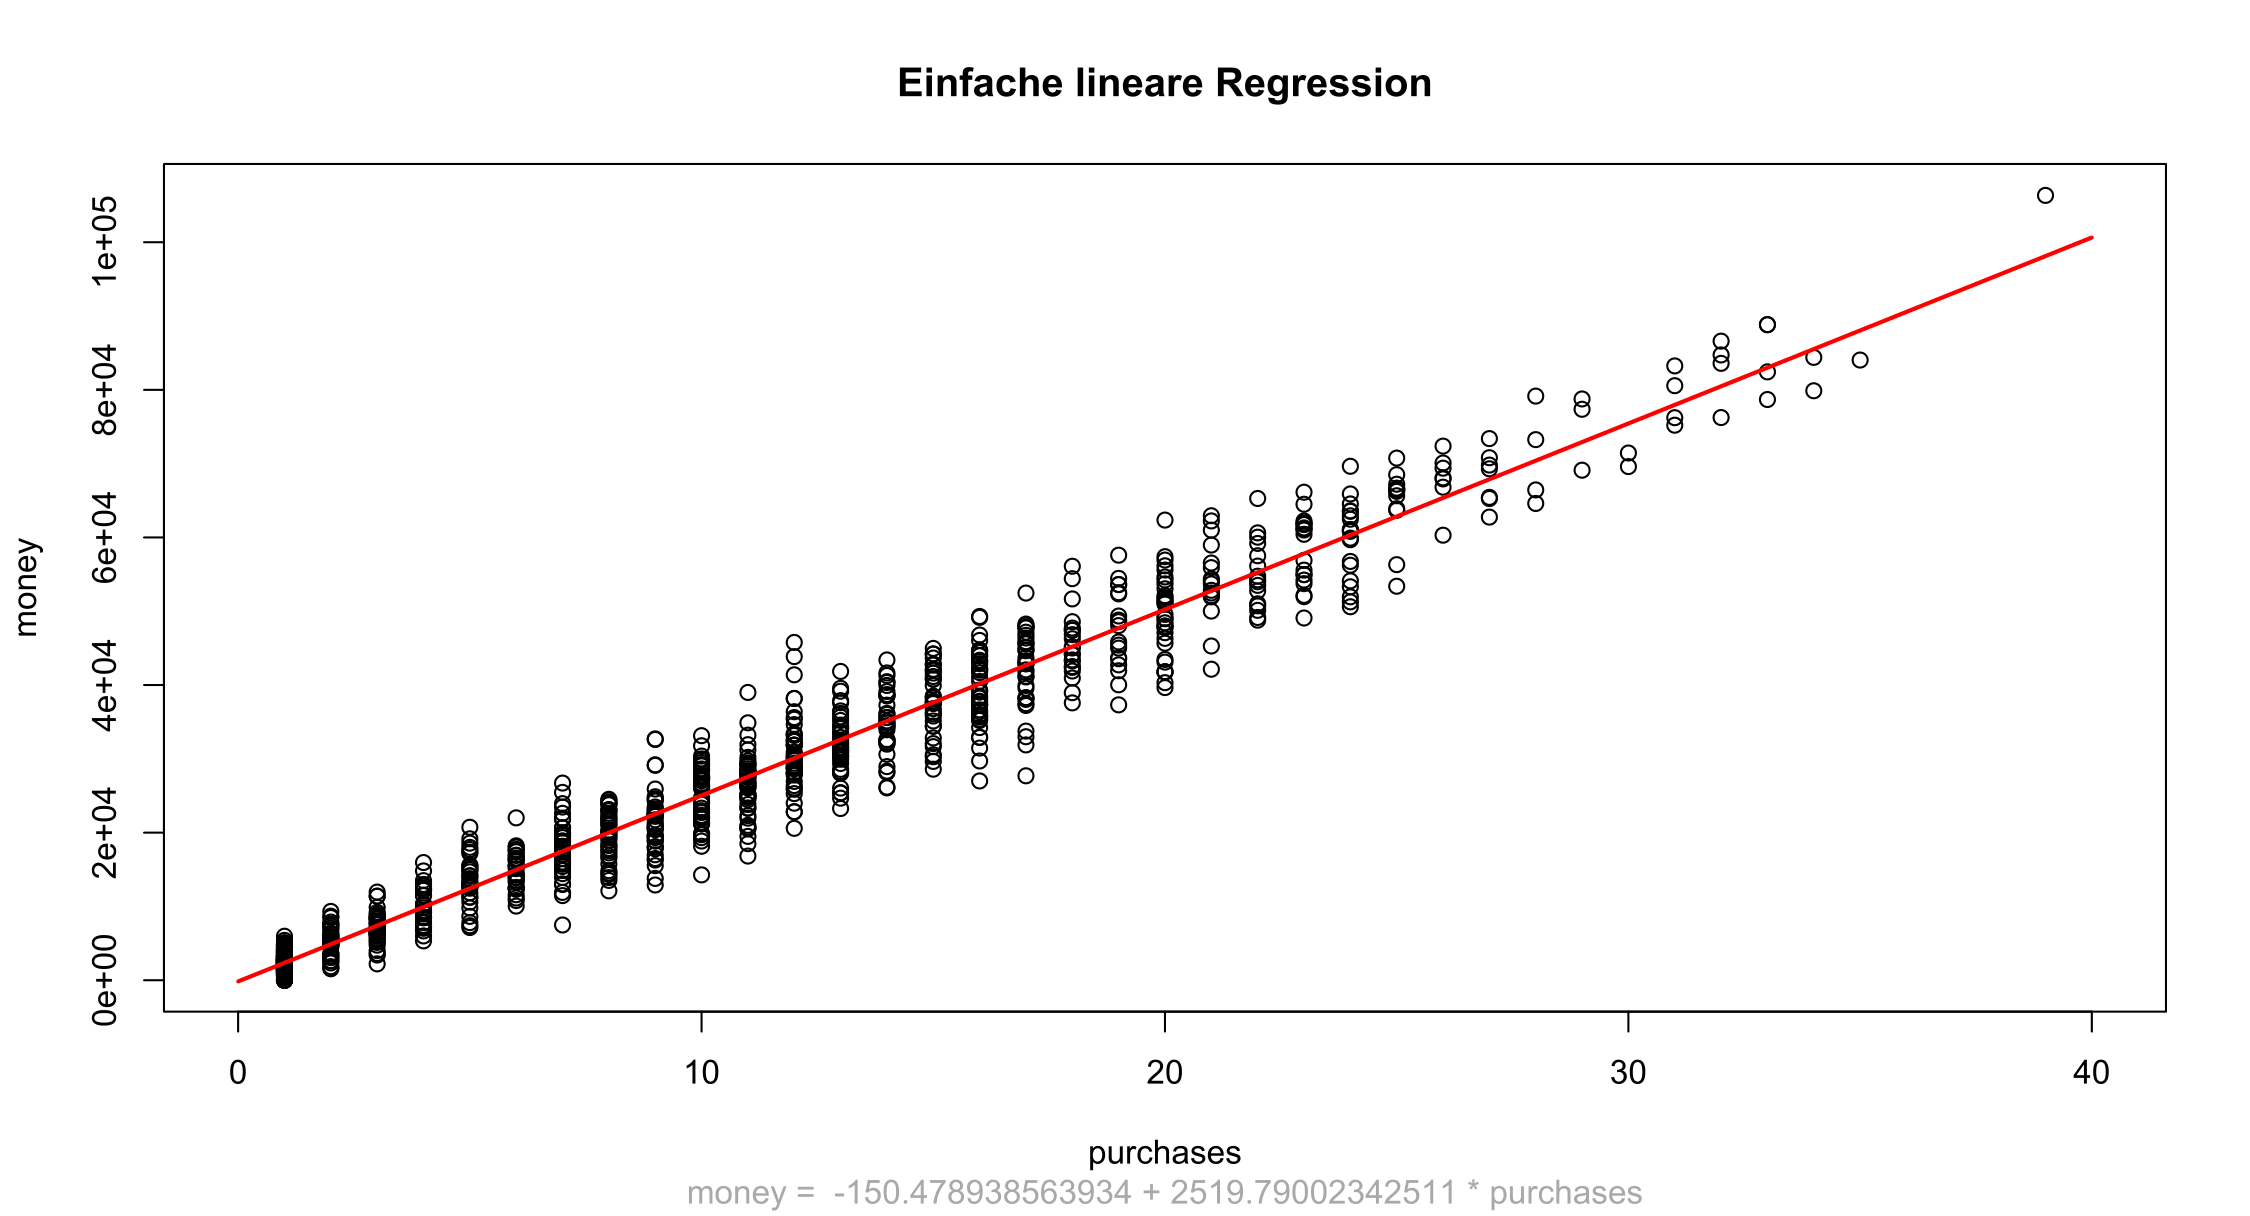
\includegraphics[width=\textwidth]{r-simpleLinearRegression}

\subsection{Multiple lineare Regression}
\label{subsection:3:2:3}

Bei multipler lineare Regression unterscheidet sich der R-Code nur in der Wahl der Formel von dem Code aus dem vorherigen Teilkapitel. Hier wollen wir $money$ durch eine lineare Summe von $purchases$ und $age$ modellieren, deshalb lautet die Formel hier "$money \sim purchases + age$". Man erhält hier das folgende Ergebnis.

\begin{minted}[linenos,breaklines,frame=single]{r}
  Coefficients:
  (Intercept)    purchases          age
       -766.7       2520.3         17.5
\end{minted}

Der Wert für $\alpha$ ist wieder relativ klein, der Wert für das $\beta$ zu $purchases$ ist fast exakt derselbe wie bei einfacher linerarer Regression, was bei denselben Daten auch zu erwarten war. Der Wert für das $\beta$ zu $age$ ist dagegen nahe bei null. Das bedeutet, dass das Alter im Vergleich zu der Anzahl der Käufe keinen signifikanten Einfluss auf das ausgegebene Geld hat.

\subsection{Logistische Regression}
\label{subsection:3:2:4}

Bei logistischer Regression nutzen wir nun nicht mehr ein lineares Modell wie bisher, sondern ein generalisiertes lineares Modell. Logistische Regression ist im Wesentlichen ein Spezialfall dieses Modelles. Hier nutzen wir also die $glm$-Funktion. Um logistische Regression damit betreiben zu können, wählt man den Parameter $family$ dieser Funktion als $binomial$.

Man braucht wie auch bei linearer Regression ein Formel für das Modell. Diese bildet man analog wie bisher, indem mal die abhängige Variable mit den unabhängigen Variablen über eine Tilde verbindet. Im Fall unserer dritten Fragestellung wählt man also die Formel als "$premium \sim money$".

Der gesamte R-Code für die logistische Regression ist wieder ähnlich zu dem Code aus \ref{subsection:3:2:1} und lautet wiefolgt:

\begin{minted}[linenos,breaklines,frame=single]{r}
  data <- read.csv2("sample.csv", sep = ",", header = TRUE)
  modell <- as.formula("premium ~ money")
  logit <- glm(modell, family = binomial, data = data)
  print(logit)
\end{minted}

Nach der Ausführung erhält man das folgende Ergebnis:

\begin{minted}[linenos,breaklines,frame=single]{r}
  Coefficients:
  (Intercept)        money
   -1.9910911    0.0000803

  Degrees of Freedom: 999 Total (i.e. Null);  998 Residual
  Null Deviance:	    1386
  Residual Deviance: 1006 	AIC: 1010
\end{minted}

Eine anschauliche Interpretation der zurückgegebenen Parameter ist nicht mehr so einfach. Wir lassen uns das Ergebnis daher wieder als Plot visualisieren:

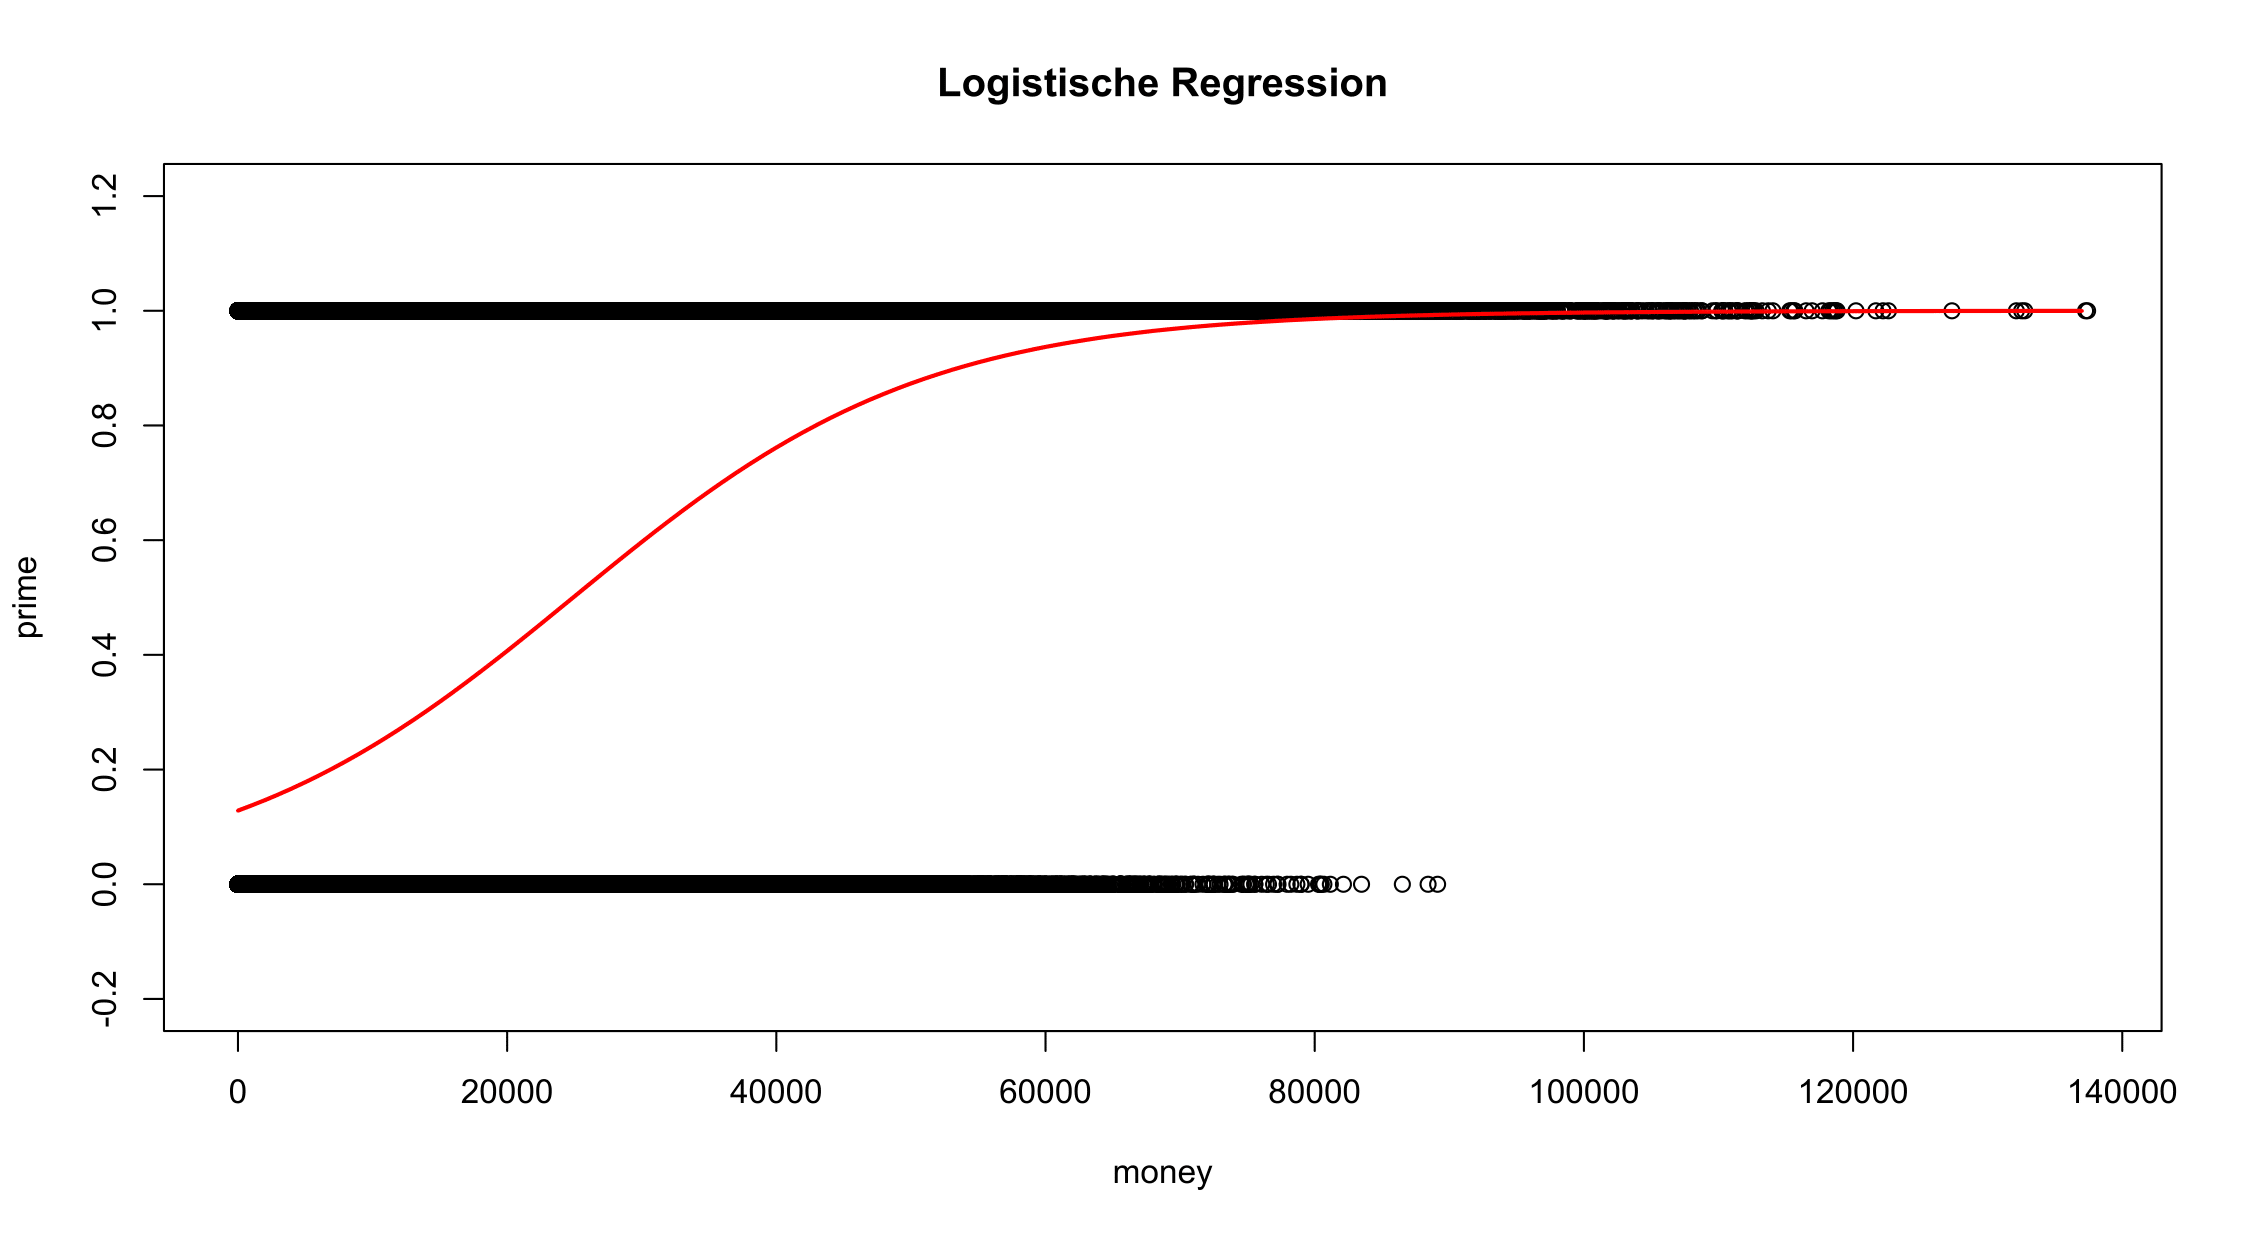
\includegraphics[width=\textwidth]{r-logisticRegression}

Für Kunden, die weniger als $100$ Euro ausgegeben haben ist die Wahrscheinlichkeit Premium-Mitglied zu sein mit etwa $25\%$ relativ gering. Je höher die Summe aber wird, desto größer wird auch die genannte Wahrscheinlichkeit. So ist ein Kunde mit mehr als $800$ Euro Ausgaben so gut wie immer ein Premium-Mitglied.

\section{TensorFlow}
\label{section:3:3}

TensorFlow ist eine Software-Bibliothek, die von Google für die Umsetzung von Algorithmen für maschinelles Lernen entwickelt wurde. Das umfasst insbesondere auch die Möglichkeit zur iterativen Optimierung von Kostenfunktionen, was wir nun zur Regressionsanalyse nutzen wollen.

TensorFlow bietet APIs für verschiedene Programmiersprachen an. Die Skripte, welche für dieser Arbeit erstellt wurden, sind in Python geschrieben. Wir verwenden TensorFlows Implementierung eines Gradientenabstiegsverfahrens, für welches man die Anzahl der Schritte und die Abstiegsgeschwindigkeit selbst wählen muss. Die Genauigkeit des Ergebnisses hängt also zusätzlich von einer angemessenen Auswahl dieser Werte ab.

Die Python-Skripte umfassen nun zwischen 70 und 100 Codezeilen, daher findet man diese Skripte im Ganzen nur im Anhang \ref{appendix:B}. Die wichtigsten Ausschnitte aus dem Code sollen in den folgenden Teilkapiteln aber einen Einblick in die Funktioneweise des Codes geben.

\subsection{Grundprinzip}
\label{subsection:3:3:1}

TensorFlow arbeitet mit Tensoren als grundliegende Datenstruktur. Solche sind im Wesentlichen Matrizen mit festen Dimensionen. Tensoren können dann mit Hilfe verschiedenster Operatoren weiterverarbeitet werden.

Es gibt drei Möglichkeiten, Tensoren zu definieren: Als Konstante, als Variable oder als Platzhalter. Während Konstanten ihren Wert nicht mehr ändern können, sind die beiden letztgenannten veränderbar. Der Unterschied besteht darin, dass Variablen mit einem Startwert initiiert werden, Platzhalter besitzen dagegen anfangs keinen Wert. Wir werden Variablen nutzen, um die Parameter über die Iterationen zu speichern. Die Daten, mit denen wir das Modell trainieren werden, übergeben wir an Platzhalter.

Wie das Modell exakt definiert wird, zeigen die folgenden Teilkapitel. Wir stellen immer eine Kostenfunktion auf, die dann mit Hilfe eines Gradientenabstiegsverfahrens iterativ minimiert wird. Die Definition dieses sogenannten Trainingsschrittes sieht immer gleich aus:

\begin{minted}[linenos,breaklines,frame=single]{python}
  train_step = tf.train
                 .GradientDescentOptimizer(learn_rate)
                 .minimize(cost)
\end{minted}

Dabei ist $tf$ die importierte TensorFlow-Bibliothek, $learn\_rate$ ist die Geschwindigkeit bzw. Schrittweite des Verfahrens und $cost$ ist die zuvor definierte Kostenfunktion.

Um dann auch wirklich Berechnungen durchführen zu können, muss in TensorFlow eine Session erzeugt werden. In dieser Session wird dann die Iteration gestartet, die $train\_step$ immer wieder mit echten Daten füttert. Je mehr Iterationen durchlaufen werden, desto exakter werden die Parameter berechnet.

\subsection{Einfache lineare Regression}
\label{subsection:3:3:2}

Hier definieren wir unsere Platzhalter und Variablen wiefolgt:

\begin{minted}[linenos,breaklines,frame=single]{python}
  x = tf.placeholder(tf.float32, [None, 1])
  y = tf.placeholder(tf.float32, [None, 1])
  alpha = tf.Variable(tf.zeros([1]))
  beta = tf.Variable(tf.zeros([1, 1]))
\end{minted}

$x$ und $y$ sind die Platzhalter für die Beispieldatensätze für das später folgende Training. $alpha$ und $beta$ sind die Parameter-Variablen, welche mit Werten null initiiert werden. Daraus berechnen wir über den linearen funktionalen Zusammenhang die geschätzten $y$ Werte:

\begin{minted}[linenos,breaklines,frame=single]{python}
  y_calc = tf.matmul(x, beta) + alpha
\end{minted}

Die Funktion $tf.matmul$ führt Matrizenmultiplikation durch. Nun definieren wir noch die Kostenfunktion als Mittelwert der Quadrate zwischen den wahren und geschätzten $y$-Werten:

\begin{minted}[linenos,breaklines,frame=single]{python}
  cost = tf.reduce_mean(tf.square(y - y_calc))
\end{minted}

Damit können wir die Session starten und unsere Parameter berechnen lassen. Mit einer Schrittweite von $0.0054$ und $2000$ Iterationen erhält man folgendes Ergebnis:

\begin{minted}[linenos,breaklines,frame=single]{python}
  alpha:  -150.377670
  beta:   2519.784424
  cost:   15031988.000000
\end{minted}

Die hier berechneten Werte für $alpha$ und $beta$ sind schon sehr nahe an den exakten Werten. Zusätzlich geben wir hier auch den aktuellen Wert der Kostenfunktion aus.

\subsection{Multiple lineare Regression}
\label{subsection:3:3:3}

Nachdem in diesem Fall nun mehr unabhängige Variablen vorhanden sind, vergrößern wir die Dimension der Tensoren $x$ und $beta$ um eins.

\begin{minted}[linenos,breaklines,frame=single]{python}
  x = tf.placeholder(tf.float32, [None, 2])
  beta = tf.Variable(tf.zeros([2, 1]))
\end{minted}

Die restlichen Variablen werden wie bei einfacher linearer Regression definiert. Das Gradientenverfahren ist bei zwei abhängigen Variablen nun komplexer, daher muss die Schrittweite verringert werden. Eine Folge davon ist, dass man mehr Schritte für dieselbe Präzision des Ergebnisses durchführen muss. Bei einer Schrittweite von $0.00071$ und $50000$ Schritten erhält man folgendes Ergebnis:

\begin{minted}[linenos,breaklines,frame=single]{python}
  alpha:           -754.910095
  beta_purchases:  2520.172363
  beta_age:        17.224550
  cost:            15004541.000000
\end{minted}

\subsection{Logistische Regression}
\label{subsection:3:3:4}

Wir definieren unsere Tensoren exakt wie bei einfacher linearer Regression, da wie hier wieder mit je einer unabhängigen und einer abhängigen Variablen arbeiten. Die bisher verwendete Berechnung der $y$-Werte fügen wir nun zusätzlich in die logistische Funktion ein:

\begin{minted}[linenos,breaklines,frame=single]{python}
  y_calc = 1 / (1 + tf.exp(- tf.matmul(x, beta) - alpha))
\end{minted}

Hier minimieren wir nicht mehr die Summe der Quadrate sondern maximieren die Likelihoodfunktion. TensorFlow bietet allerdings nur eine API für Minimierung, weshalb wir das Inverse der Likelihoodfunktion als Kostenfunktion verwenden. Zusätzlich wenden wir wieder den natürlichen Logarithmus auf die Funktion an. Die Kostenfunktion sieht also wie folgt aus:

\begin{minted}[linenos,breaklines,frame=single]{python}
  cost = - tf.reduce_sum(
    tf.log(
      y * y_calc +
      (1 - y) * (1 - y_calc)
    )
  )
\end{minted}

Wir wählen eine Schrittweite von $0.0001$ und iterieren $1000$ Schritte, um das folgende Ergebnis zu erhalten:

\begin{minted}[linenos,breaklines,frame=single]{python}
  alpha:  -1.991089
  beta:   0.000080
  cost:   502.972290
\end{minted}

\section{SQL}
\label{section:3:4}

Die "Structured Query Language" alias "SQL" ist eine Sprache zur Definition und Verarbeitung von Datenstrukturen in Datenbanksystemen und wird in nahezu allen Implementierungen relationaler Datenbanken unterstützt. Oft liegen die Daten, welche man für Regressionsanalyse verwenden möchte in einer solchen Datenbank.

SQL als Programmiersprache ist Turing-vollständig. Es ist also mit standardisierten SQL-Methoden möglich, Regression direkt in der Datenbank zu betreiben. Die konkrete Umsetzung hängt von der Art der Regression und dem spezifischen Datenbanksystem ab. In diesem Kapitel soll das nun für zwei Open-Source-Datenbanksystemen demonstriert werden, nämlich MySQL und PostgreSQL. Der vollständige SQL-Code befindet sich wegen der Länge wieder komplett im Anhang. Die MySQL-Skripte sind unter \ref{appendix:C} zu finden, die Skripte für PostgreSQL liegen in \ref{appendix:D}.

Im Gegensatz zu den beiden bisher vorgestellten Sprachen verfolgen wir hier kein einheitliches Grundprinzip, in dem sich alle Arten der Regression ähnlich sind. Die einzige Gemeinsamkeit ist, dass wir in allen SQL-Skripten Prozeduren bzw. Funktionen definieren, welche bei Aufruf die Regressionsanalyse durchführen. Wir nehmen dazu an, dass die Daten für die Regression in einer Tabelle namens $sample$ liegen.

Bei einfacher linearer Regression berechnen wir die Parameter exakt über die Formeln aus Kapitel \ref{subsection:2:1:1}. Bei multipler Regression verwenden wir die Matrixformel aus Kapitel \ref{subsection:2:1:2}. Hier müssen wir zusätzlich Algorithmen zur Transponierung, Multiplikation und Invertierung von Matrizen implementieren. Für logistische Regression steht uns keine explitize Formel zur Verfügung, weshalb wir ein Gradientenverfahren zur Lösung des Optimierungsproblems implementieren.

\subsection{Einfache lineare Regression}
\label{subsection:3:4:1}

Einfache lineare Regression kann ohne größeren Aufwand mit SQL umgesetzt werden. Wir berechnen zuerst die Mittelwerte über die Spalten $purchases$ und $money$, dann die Summen in Zähler und Nenner der Formel für $\beta$ und können dann mit einfacher Arithmetik die beiden Paramter bestimmen.

Diese Berechnung kann man sogar in einer einzelnen Abfrage umsetzen. Das Skript für PostgreSQL tut das auch und definiert die genannten Berechnungsschritte als einzelne Views. In MySQL existiert die VIEW-Syntax nicht. Deshalb wird die Berechnung der Übersicht halber auf mehrere Abfragen aufgeteilt.

Führen wir die Prozeduren im jeweiligen Datenbanksystem aus, erhalten wir folgende Ergebnisse:

\begin{center}
  \captionof{table}{Einfache lineare Regression in MySQL}
  \begin{tabular}{|c|c|}\hline
    \textbf{variable} & \textbf{value} \\ \hline
    alpha & -150.47893856389208170000 \\ \hline
    beta & 2519.79002342511470000000 \\ \hline
  \end{tabular}

  \captionof{table}{Einfache lineare Regression in PostgreSQL}
  \begin{tabular}{|c|c|}\hline
    \textbf{variable} & \textbf{value} \\ \hline
    alpha & -150.47893856381151146861740350360640000000000000 \\ \hline
    beta & 2519.7900234251071069143923667424 \\ \hline
  \end{tabular}
\end{center}

\subsection{Multiple lineare Regression}
\label{subsection:3:4:2}

Wir wollen zur Lösung dieses Regressionsproblems die Matrix-Formel aus Kapitel \ref{subsection:2:1:2} anwenden. Dazu müssen Methoden für das Transponieren, Multiplizieren und Invertieren von Matrizen implementiert werden, da weder MySQL noch PostgreSQL über solche Funktionen verfügen. Wir müssen außerdem einen Weg finden, Matrizen im jeweiligen Datenbanksystem zu repräsentieren.

Die Matrizenrepräsentierung lösen wir unterschiedlich in den beiden Datenbanksystemen. In MySQL definieren wir uns temporäre Tabellen, welche jeweils eine Matrix repräsentieren. Jede solche Tabelle besitzt dasselbe Schema, nämlich aus den Attributen $row$, $column$ und $value$. Die ersten beiden enthalten die Indizes des Matrixelements, letztere enthält den Wert des jeweiligen Elements.

Wir definieren insgesamt sieben solcher Tabellen:
\begin{itemize}
  \item $matrix\_X$: Entspricht der Matrix $X$ aus der Berechnungsformel.
  \item $matrix\_y$: Entspricht der Matrix $y$ aus der Berechnungsformel.
  \item $matrix\_transposed$: Entspricht der Matrix $X^T$.
  \item $matrix\_product\_1$: Entspricht dem Matrixprodukt $X^T X$.
  \item $matrix\_inverse$: Entspricht dem Inversen des obigen Matrixprodukts $(X^T X)^{-1}$.
  \item $matrix\_product\_2$: Entspricht dem Matrixprodukt $X^T y$.
  \item $matrix\_result$: Entspricht dem Endergebnis der Berechnungsformel $(X^T X)^{-1} X^T y$.
\end{itemize}

Die ersten beiden dieser Tabellen werden einfach mit den vorhandenen Werten aus der Tabelle $sample$ befüllt. Die Tabelle $matrix\_transposed$ wird mit einem einfachen Query aus der Tabelle $matrix\_X$ berechnet, indem die Indizes für Zeile und Spalte vertauscht werden.

Die Tabellen $matrix\_product\_1$, $matrix\_product\_2$ und $matrix\_result$ sind Ergebnisse von Matrizenmultiplikationen. Diese Produkte werden mit zwei Schleifen berechnet, die über die Tupel und Attribute der Ergebnismatrix iterieren. Der jeweilige Wert zusammen mit dem Zeilen- und Spaltenindex der zu berechnenden Matrix wird über eine Abfrage eingefügt. Diese Abfrage nimmt das Kreuzprodukt beider Tabellen und betrachtet nur die aktuelle Zeile der ersten Tabelle und die aktuelle Spalte der zweiten Tabelle. Außerdem sollen die Zeilenindizes der ersten Tabelle gleich den Indizes der zweiten Tabelle sein. Der Wert für die zu berechnende Matrix ergibt sich als Summe über die Produkte der Werte der verbleibenden Tupel.

Bei den Tabellen $matrix\_product\_2$ und $matrix\_result$ ist die Spaltenanzahl der zu berechnenden Tabelle gleich eins. Wegen der einen notwendigen Iteration braucht man hier sogar nur eine Schleife.

Für die Berechnung der inversen Matrix, also für die Tabelle $matrix\_inverse$, wird ein einfacher iterativer Algorithmus verwendet, welcher über alle Zeilen der zu invertierenden Matrix läuft. In jedem Schritt werden alle Elemente der Matrix nach einem bestimmten Vorgehen angepasst, sodass man am Ende das Inverse erhält. Details zu dem verwendeten Algorithmus findet man in \cite{matrix}.

Die komplette Berechnung wurde in eine Prozedur verpackt. Führt man diese aus, erhält man das folgende Ergebnis:

\begin{center}
  \captionof{table}{Multiple lineare Regression in MySQL}
  \begin{tabular}{|c|c|}\hline
    \textbf{variable} & \textbf{value} \\ \hline
    alpha & -766.73617378441900469987 \\ \hline
    beta\_purchases & 2520.30174179130808582094 \\ \hline
    beta\_age & 17.50372214336084692771 \\ \hline
  \end{tabular}
\end{center}

Betrachten wir nun die Implementierung in PostgreSQL. Gegenüber MySQL hat man hier den Vorteil, dass mehrdimensionale Felder als Datentyp existieren. Wir brauchen also keine temporären Tabellen für die Matrizen mehr, sondern speichern diese einfach als zweidimensionales Array.

Neben der eigentlichen Prozedur zum Ausführen der Regression definieren wir drei weitere Funktionen:
\begin{itemize}
  \item $matrix\_transpose$: Diese Funktion nimmt ein zweidimensionales Array von Typ $NUMERIC$ als Input und gibt die transponierte Matrix zurück. Die transponierte Matrix wird mit zwei Schleifen über die Zeilen und Spalten gebildet, welche die Zeilen- und Spaltenindizes vertauschen.
  \item $matrix\_multiplication$: Diese Funktion nimmt zwei zweidimensionale Arrays vom Typ $NUMERIC$ als Input und gibt das Produkt der beiden Matrizen zurück. Hier werden drei Schleifen zur Berechnung verwendet. Die ersten beiden iterieren über die Zeilen und Spalten der Ausgabematrix. Die dritte iteriert über die Zeile bzw. Spalte, welche zur Berechnung der aktuellen Elements verwendet werden und addiert die Produkte der Elemente dieser Zeile und Spalte auf.
  \item $matrix\_inversion$: Diese Funktion nimmt ein zweidimensionales Array vom Typ $NUMERIC$ als Input und gibt das Inverse dieser Matrix zurück. Dabei wird derselbe Algorithmus verwendet, der auch in MySQL implementiert wurde.
\end{itemize}

Mit diesen drei Funktionen lässt sich die Formel aus Kapitel \ref{subsection:2:1:2} mit drei Abfragen umsetzen. Dazu erzeugen wir zuerst zwei Matrizen $x$ und $y$ mit den unabhängigen und der abhängigen Variable als Elemente aus der $sample$-Relation. Im dritten Query nutzen wir die genannten Funktionen, um die Matrix mit den gesuchten Parametern zu berechnen.

Führt man die multiple lineare Regressionsanalyse in PostgreSQL durch, erhält man das folgende Ergebnis:

\begin{center}
  \captionof{table}{Multiple lineare Regression in PostgreSQL}
  \begin{tabular}{|c|c|}\hline
    \textbf{variable} & \textbf{value} \\ \hline
    alpha & -766.73617378441900469987 \\ \hline
    beta\_purchases & 2520.30174179130808582094 \\ \hline
    beta\_age & 17.50372214336084692771 \\ \hline
  \end{tabular}
\end{center}

Da wir dieselben Algorithmen und dieselbe Präzision für Kommazahlen in MySQL und PostgreSQL verwendet haben, stimmen die beiden Ergebnisse sogar überein.

\subsection{Logistische Regression}
\label{subsection:3:4:3}

Zur Lösung des logistischen Regressionsproblems möchten wir in SQL ein Gradientenverfahren implementieren. Wir verwenden denselben Algorithmus in MySQL und PostgreSQL, das heißt die Skripte unterscheiden sich lediglich in der datenbankspezifischen Syntax.

Wir verwenden für das Verfahren mehrere Tabellen, in denen gewisse Informationen gespeichert und verarbeiten werden:
\begin{itemize}
  \item Die Relation $datapoints$ besteht aus drei Spalten $id$, $variable$ und $value$. Die $id$-Spalte enthält einen generierten Wert, der einen Datensatz aus der $sample$-Tabelle identifiziert. Die $variable$-Spalte enthält den Namen der gespeicherten unabhängigen Variable. In unserem Fall steht hier immer $beta\_money$, da wir nur eine unabhängige Variable betrachten. Gegebenenfalls können hier mehrere Variablen betrachtet werden. (Die Werte für einen Datenpunkt werden dann also auf mehrere Zeilen aufgeteilt.) Die Spalte $value$ enthält dann den Wert der entsprechenden Variable des jeweiligen Datensatzes.
  \item Die Relation $binary\_values$ besteht aus zwei Spalten $id$ und $value$. Hier werden für jeden Datenpunkt die Werte der abhängigen binären Variable gespeichert, in unserem Fall also die Werte aus der Spalte $premium$.
  \item Die Relation $parameters$ besteht aus drei Spalten $variable$, $old$ und $new$. Die erste Spalte enthält den Namen des Parameters, also $alpha$ oder $beta\_money$. Die Spalten $old$ und $new$ enthalten die Werte der Parameter vor bzw. nach dem aktuellen Iterationsschritt des Gradientenverfahrens. Wir benötigen beide Werte, um überprüfen zu können, ob die neuen Parameter ein besseres Ergebnis liefern als die alten.
  \item Die Relation $logits$ besteht aus drei Spalten $id$, $old$ und $new$. Hier werden für jeden Datenpunkt die Werte der logistischen Funktion $\pi_i$ berechnet. Dabei werden einmal die alten und einmal die neuen Parameter zur Berechnung verwendet.
  \item Die Relation $gradient$ besteht aus zwei Spalten $variable$ und $value$. Hier wird der Gradient bzw. die Werte der partiellen Ableitungen nach jedem Parameter gespeichert.
\end{itemize}

Wir definieren außerdem einige Hilfsfunktionen:
\begin{itemize}
  \item $calculate\_logits$: Diese Funktion berechnet die Werte für die logistische Funktion für alle Datenpunkte und trägt diese in die Tabelle $logit$ ein. Dabei wird die Funktion für beide Parameterwerte ($old$ und $new$) aus der Tabelle $parameters$ berechnet.
  \item $calculate\_gradient$: Diese Funktion berechnet den Gradienten auf Basis der alten Parameterwerte und der Werte der logistischen Funktion aus der Tabelle $logits$.
  \item $calculate\_parameters$: Diese Funktion nimmt eine Schrittweite als Argument, berechnet daraus und aus den Werten der $gradient$-Tabelle die neuen Parameter und schreibt diese zurück in die Spalte $new$ der Tabelle $parameters$.
  \item $are\_new\_parameters\_better$: Diese Funktion berechnet den Logarithmus der Likelihoodfunktion für die neuen und alten Parameter aus der Tabelle $parameters$ und gibt einen Wahrheitswert zurück. Die Rückgabe ist wahr, wenn die Likelihoodfunktion für die neuen Parameter einen größeren Wert annimmt als für die alten Parameter.
\end{itemize}

Wir führen wie schon bei TensorFlow zuerst eine Lineartransformation für die Werte aus $money$ durch und bilden diese linear auf das Interval $[0, 1]$ ab. Das dient erneut dazu, dass die Werte der logistischen Funktion nicht zu nahe an null geraten. Die transformierten Werte fügen wir in die $datapoints$-Tabelle ein. Auch die anderen Tabellen erzeugen wir und fügen initiale Werte ein.

Es folgt eine $while$-Schleife, die solange läuft, bis entweder die vorgegebene Anzahl an Schritten erreicht wurde, oder die Schrittweite zu klein für die gewählte Präzision der Kommazahlen wird. Wir berechnen zuerst den Gradienten, dann die neuen Parameter. Dann ist ein Aufruf von $calculate\_logits$ nötig, um die logistische Funktion für die neuen Parameter zu berechnen.

Wir überprüfen, ob die neuen Parameter wirklich besser sind als die alten. Falls nicht, wird die Schrittweite halbiert, danach werden die Parameter und die Werte der logistischen Funktion erneut berechnet. Das wird solange wiederholt, bis die neuen Parameter besser sind oder die Schrittweite unter die Präzisionsgrenze fällt.

Haben wir die neuen Parameter erfolgreich berechnet, werden die Werte der $old$-Spalten in den Tabellen $parameters$ und $logits$ mit den neuen Werten überschrieben und der Iterationsschritt ist beendet. Nachdem die Schleife beendet wurde, werden die Parameter wieder entsprechend linear transformiert, um den tatsächlichen Werten für $money$ zu entsprechen.

Wir entscheiden und für 1000 Iterationen und wählen eine Schrittweite von $0.00008$. Führt man die Prozeduren im jeweiligen Datenbanksystemen aus erhält man das folgende Ergebnis:

\begin{center}
  \captionof{table}{Logistische Regression in MySQL}
  \begin{tabular}{|c|c|}\hline
    \textbf{variable} & \textbf{value} \\ \hline
    alpha & -1.991090115311453143480846099933 \\ \hline
    beta\_money & 0.000080298536993602280846099933 \\ \hline
  \end{tabular}

  \captionof{table}{Logistische Regression in PostgreSQL}
  \begin{tabular}{|c|c|}\hline
    \textbf{variable} & \textbf{value} \\ \hline
    beta\_money & 0.000080298565326972737807097397 \\ \hline
    alpha & -1.991090799730035106155287378451 \\ \hline
  \end{tabular}
\end{center}


\chapter{Vergleich der verschiedenen Implementierungen}
\label{chapter:4}

In diesem Kapitel wollen wir zum einen konkret auf die Unterschiede eingehen und zum anderen die Laufzeit abhängig von der Anzahl der zu verarbeitenden Datensätze evaluieren.

\section{Benchmarking}
\label{section:4:1}

Nun wollen wir die konkreten Laufzeiten für die implementierten Algorithmen vergleichen. Zu erwarten ist auf jeden Fall, dass Skripte unter Verwendung von iterativen Verfahren länger laufen als solche mit expliziter Berechnung.

Zur Berechnung der Laufzeiten erfolgt erneut mit einem Python-Skript. Dieses Skript führt die jeweilige Regression über einen Kommandozeilenbefehl aus und misst die Zeit dieser Operation. Die Anzahl der Wiederholungen und die Anzahl der verwendeten Datenpunkte können als Parameter übergeben werden. Die Ergebnisse der Berechnungen werden als csv-Datei gespeichert. Das Skript findet man im Anhang unter \ref{appendix:F:1}.

Auch für das Auswerten der berechneten Benchmarks wurde ein Python-Skript erstellt. Dieses Skript liest eine csv-Datei mit Benchmarks und gibt eine Tabelle mit den Werten für jede Art der Regression aus. Außerdem werden mehrere Plots für die Laufzeiten erzeugt. Alle Benchmarks wurden auf einem MacBook Pro (Mitte 2012, Betriebssystem macOS High Sierra 10.13.2) mit einem 2,9 GHz Intel Core i7 Prozessor und 8 GB 1600 MHz DDR3 Arbeitsspeicher berechnet.

\subsection{Einfache lineare Regression}
\label{subsection:4:1:1}

Folgende Ergebnisse erhalten wir bei einfacher linearer Regression:

\begin{center}
  \captionof{table}{Laufzeiten für einfache lineare Regression}
  \begin{tabular}{|c|c|c|c|c|c|}\hline
    & \textbf{10} & \textbf{100} & \textbf{1000} & \textbf{10000} & \textbf{100000} \\ \hline
    \textbf{r} & 0.38453477 & 0.40336191 & 0.38638819 & 0.40475887 & 0.54730985 \\ \hline
    \textbf{tensorflow} & 2.96190362 & 2.94665535 & 3.00290149 & 3.69807061 & 7.73616447 \\ \hline
    \textbf{mysql} & 0.02591379 & 0.02506811 & 0.03348756 & 0.11362195 & 0.82149320 \\ \hline
    \textbf{postgresql} & 0.03092405 & 0.03056195 & 0.03340294 & 0.04948901 & 0.21394655 \\ \hline
  \end{tabular}
\end{center}

Der zugehörige Graph sieht folgendermaßen aus:

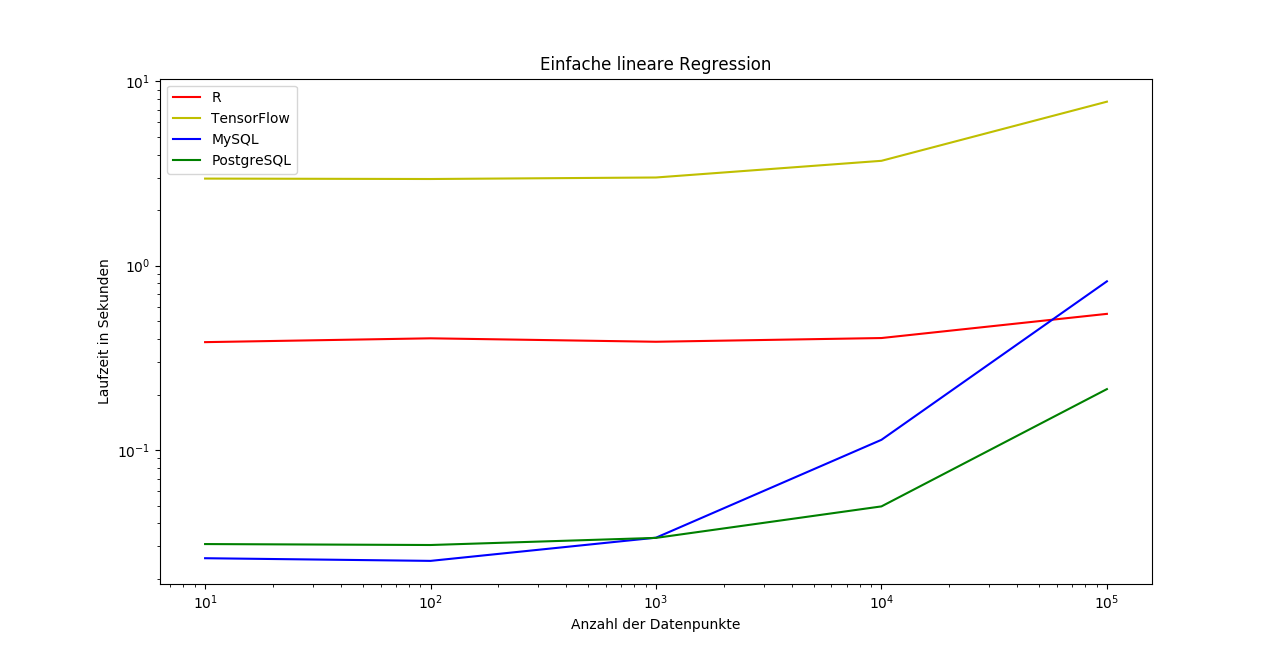
\includegraphics[width=\textwidth]{simpleLinearRegressionBenchmark}

TensorFlow und R haben eine relativ konstante Lautzeit, auch bei größeren Datenmengen. Dabei ist TensorFlow mit iterativer Berechnung wie erwartet mit Abstand am langsamsten. Die SQL-Implementierungen sind bei geringer Anzahl an Datenpunkten sogar die schnellsten Skripte. Für größer werdende Datenmengen erkennt man aber einen rapiden Anstieg in der Laufzeit.

\subsection{Multiple lineare Regression}
\label{subsection:4:1:2}

Die Skripte für multiple lineare Regression besitzen folgende Laufzeiten:

\begin{center}
  \captionof{table}{Laufzeiten für multiple lineare Regression}
  \begin{tabular}{|c|c|c|c|c|c|}\hline
    & \textbf{10} & \textbf{100} & \textbf{1000} & \textbf{10000} & \textbf{100000} \\ \hline
    \textbf{r} & 0.38108478 & 0.37967851 & 0.38452695 & 0.39888490 & 0.54517789 \\ \hline
    \textbf{tensorflow} & 167.220486 & 168.885465 & 168.668689 & 168.821214 & 169.254182 \\ \hline
    \textbf{mysql} & 0.04174929 & 0.05248516 & 0.15990342 & 1.09634777 & 10.8214030 \\ \hline
    \textbf{postgresql} & 0.03053954 & 0.03336087 & 0.05904620 & 0.30572490 & 2.71992954 \\ \hline
  \end{tabular}
\end{center}

Das geplottete Ergebnis sieht wie folgt aus:

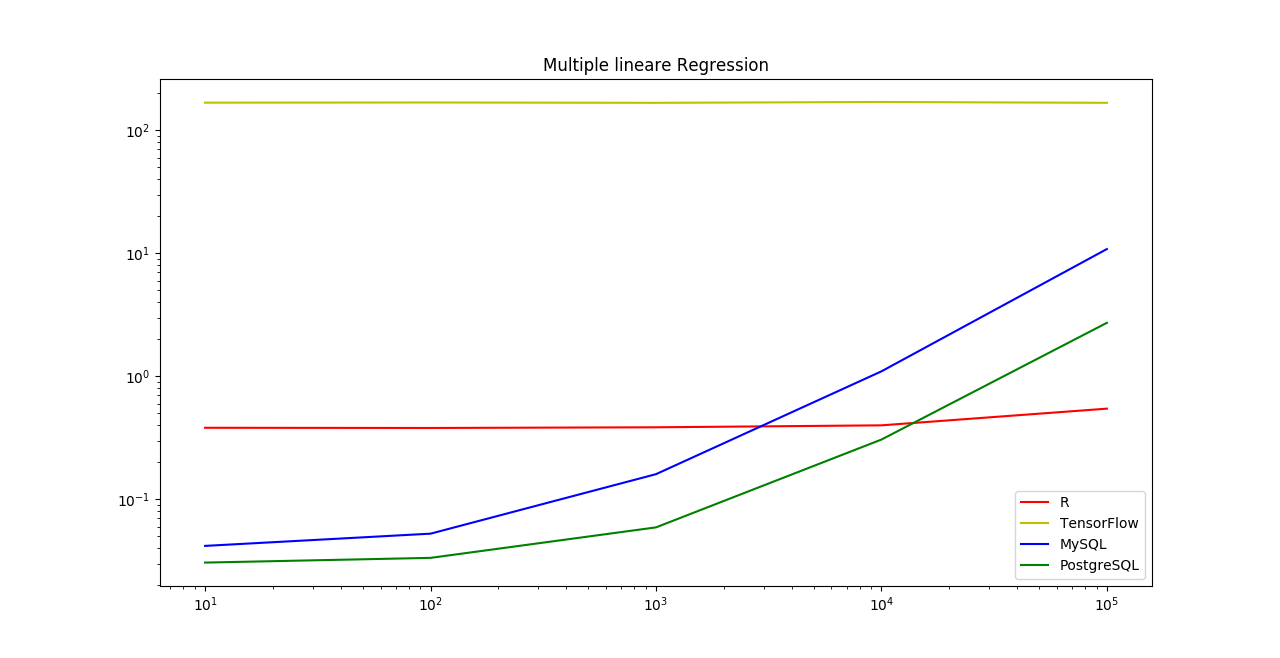
\includegraphics[width=\textwidth]{multipleLinearRegressionBenchmark}

Hier zeigt sich ein ähnliches Bild wie schon bei einfacher linearer Regression. Wieder liefern R und TensorFlow relativ konstante Laufzeiten, wobei die Laufzeit des TensorFlow-Skriptes wegen den $50.000$ durchgeführten Iterationen dieses Mal extrem langsam ist. Wieder sind die SQL-Skripte bei kleinen Datenmengen am schnellsten. Bei größeren Datenmengen werden sie allerdings von R geschlagen. Interessant ist außerdem, dass die PostgreSQL-Implementierung noch schneller als die Variante in MySQL. Die Arrays von PostgreSQL arbeiten also effizienter als die temporären Relationen in MySQL.

\subsection{Logistische Regression}
\label{subsection:4:1:3}

Betrachten wir zuletzt noch die Laufzeiten für logistische Regression:

\begin{center}
  \captionof{table}{Benchmarks für logistische Regression}
  \begin{tabular}{|c|c|c|c|c|c|}\hline
    & \textbf{10} & \textbf{100} & \textbf{1000} & \textbf{10000} & \textbf{100000} \\ \hline
    \textbf{r} & 0.40403676 & 0.39953323 & 0.40047518 & 0.43356463 & 0.91014730 \\ \hline
    \textbf{tensorflow} & 2.88191271 & 2.88278436 & 2.92470042 & 3.37794654 & 6.87024382 \\ \hline
    \textbf{mysql} & 1.57908838 & 4.51631200 & 35.3472805 & 283.849979 & 2680.43056 \\ \hline
    \textbf{postgresql} & 3.73521209 & 48.8452754 & 521.625671 & 5175.87997 &  \\ \hline
  \end{tabular}
\end{center}

Die Visualisierung der Tabelle sieht so aus:

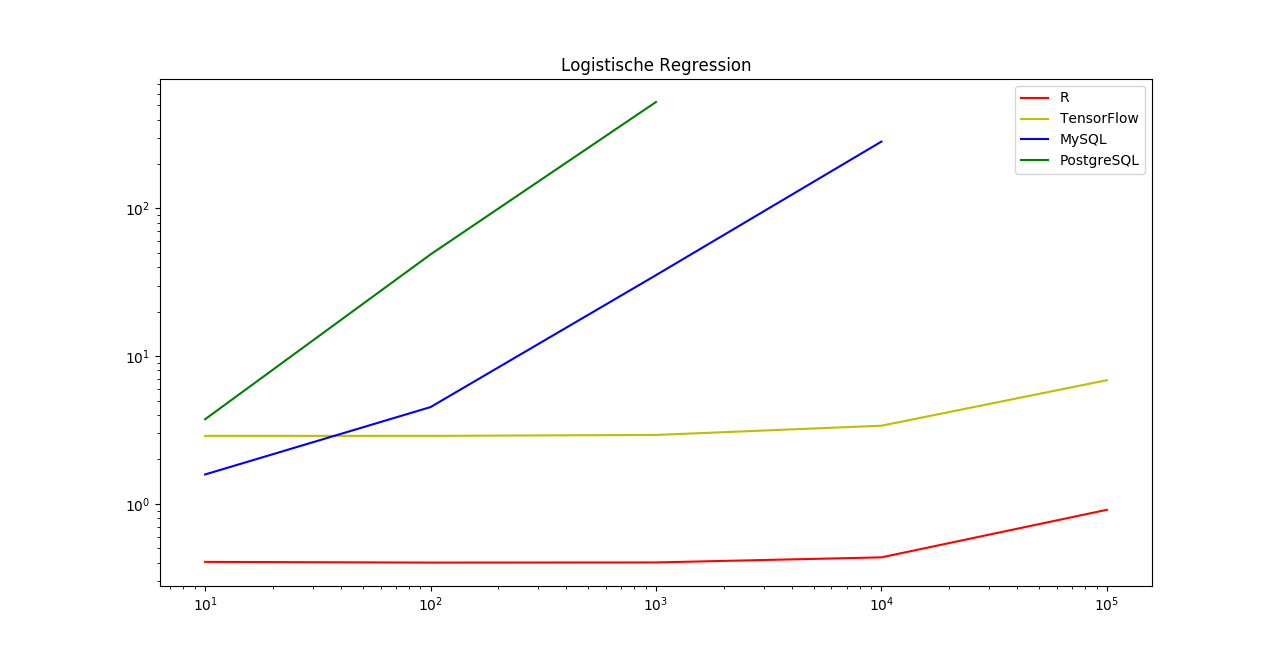
\includegraphics[width=\textwidth]{logisticRegressionBenchmark}

Wieder erkennt man eine Ähnlichkeit zu den vorherigen Diagrammen. Die SQL-Implementierungen sind nun aber von Anfang an deutlich langsamer als die Skripte in R und TensorFlow. Die Laufzeit steigt außerdem sehr schnell weiter an. So wurden für $100.000$ Datenpunkte in PostgreSQL gar keine Benchmarks mehr berechnet, da die erwartete Laufzeit etwa $50.000$ Sekunden, also knapp 14 Stunden beträgt. Klarer Gewinner ist hier R, wo auch $100.000$ Datenpunkte in weniger als einer Sekunde verarbeitet werden können.


\chapter{Erweiterungspotenzial in Datenbanksystemen}

In Kapitel \ref{section:3:4} wurde gezeigt, wie Regressionsanalyse in SQL durchgeführt werden kann. Die dazu implementierten Funktionen können als Erweiterungspotenzial für relationale Datenbanksysteme gesehen werden.

In diesen Funktionen sind die zu verwendende Relation und deren Attribute aktuell noch fest implementiert. Um diese Funktionen also nutzbar zu machen, müsste man weitere Parameter einfügen, mit denem man Relation und Attribute zum Zeitpunkt der Ausführung bestimmen kann.

Wir wollen nun die hier implementierten Funktionen und insbesondere deren Abfragen mit Hilfe von Operatorenbäumen darstellen.

\section{Einfache lineare Regression}
\label{section:5:1}

Die einfache lineare Regression besteht aus mehreren kleinen Teilabfragen. Zuerst berechnet man die Mittelwerte der beiden Attribute für die Regression. Das Ergebnis ist die Tabelle $means$:
\\\\
\noindent\fbox{\begin{minipage}{\dimexpr\textwidth-2\fboxsep-2\fboxrule\relax}
  \Tree[
    .$\rho_{mean\_purchases ~\leftarrow~ avg(purchases),~ mean\_money ~\leftarrow~ avg(money)}$
    [
      .$\gamma_{avg(purchases),~ avg(money)}$
      $datapoints$
    ]
  ]
\end{minipage}}
\\\\
Mit diesen Mittelwerten berechnet man die Summen im Nenner und Zähler der Lösungsformel für $\beta$ aus \ref{subsection:2:1:1}. Die Tabelle $sums$ ist das Ergebnis dieser Abfrage:
\\\\
\noindent\fbox{\begin{minipage}{\dimexpr\textwidth-2\fboxsep-2\fboxrule\relax}
  \Tree[
    .$\rho_{denominator ~\leftarrow~ sum(power(purchases - mean\_purchases, 2))}$
    [
      .$\rho_{nominator ~\leftarrow~ sum((purchases - mean\_purchases) \cdot (money - mean\_money))}$
      [
        .$\gamma_{sum((purchases - mean\_purchases) \cdot (money - mean\_money)),~ sum(power(purchases - mean\_purchases, 2))}$
        [
          .X
          $datapoints$
          $means$
        ]
      ]
    ]
  ]
\end{minipage}}
\\\\

Damit berechnet man einen Wert für $beta$:
\\\\
\noindent\fbox{\begin{minipage}{\dimexpr\textwidth-2\fboxsep-2\fboxrule\relax}
  \Tree[
    .$\rho_{variable ~\leftarrow~ "beta",~ value ~\leftarrow~ nominator / denominator}$
    [
      .$\pi_{"beta",~ nominator / denominator}$
      $sums$
    ]
  ]
\end{minipage}}
\\\\
Mit Hilfe von $beta$ kann man nun auch $alpha$ berechnen:
\\\\
\noindent\fbox{\begin{minipage}{\dimexpr\textwidth-2\fboxsep-2\fboxrule\relax}
  \Tree[
    .$\rho_{variable ~\leftarrow~ "alpha",~ value ~\leftarrow~ mean\_money - value \cdot mean\_purchases}$
    [
      .$\pi_{"alpha",~ mean\_money - value \cdot mean\_purchases}$
      [
        .X
        $means$
        $beta$
      ]
    ]
  ]
\end{minipage}}
\\\\

\section{Multiple lineare Regression}
\label{section:5:2}

Die hier gezeichneten Bäume entsprechen nicht der Implementierung in PostgreSQL. Dort verwenden wir Arrays und Schleifen zur Berechnung. In MySQL verwenden wir dagegen Tabellen und verarbeiten diese mit den angegebenen Bäumen.

Hier beginnen wir mit der Berechnung der transponierten Matrix von $X$. Die zugehörige Tabelle wird $matrix\_transposed$ genannt:
\\\\
\noindent\fbox{\begin{minipage}{\dimexpr\textwidth-2\fboxsep-2\fboxrule\relax}
  \Tree[
    .$\rho_{row ~\leftarrow~ column, column ~\leftarrow~ row}$
    $matrix\_X$
  ]
\end{minipage}}
\\\\
Die Matrixprodukte werden auch in MySQL mit Schleifen berechnet. Dabei wird ein Element der zu berechnenden Matrix mit folgender Abfrage bestimmt. Dabei sind die Iteratoren $counter\_1$ und $counter\_2$ durch die Schleifen gegeben
\\\\
\noindent\fbox{\begin{minipage}{\dimexpr\textwidth-2\fboxsep-2\fboxrule\relax}
% --------------------------------------------------------------
% Dieser Baum entspricht der Implementierung ohne Schleifen.
% --------------------------------------------------------------
%   \Tree[
%     .$\gamma_{matrix\_transposed.row, matrix\_X.column, sum(matrix\_transposed.value \cdot matrix\_X.value)}$
%     [
%       .$\sigma_{matrix\_transposed.column = matrix\_X.row}$
%       [
%         .X
%         $matrix\_transposed$
%         $matrix\_X$
%       ]
%     ]
%   ]
  \Tree[
    .$\gamma_{sum(m1.value \cdot m2.value)}$
    [
      .$\sigma_{m1.row = counter\_1,~ m2.column = counter\_2,~ m1.column = m2.row}$
      [
        .X
        [
          .$\rho_{m1}$
          $matrix\_transposed$
        ]
        [
          .$\rho_{m2}$
          $matrix\_X$
        ]
      ]
    ]
  ]
\end{minipage}}
\\\\
Die beiden Matrixprodukte zur Berechnung von $matrix\_product\_2$ und $matrix\_result$ besitzen denselben Operatorenbaum, nur dass die beiden Relationen $matrix\_transposed$ und $matrix\_y$ bzw. $matrix\_inverse$ und $matrix\_product\_2$ verwendet werden.

Zur Berechnung der inversen Matrix für die Relation $matrix\_inverse$ wird in PostgreSQL und MySQL ein iterativer Algorithmus verwendet, der sich nicht als Operatorenbaum darstellen lässt.

\section{Logistische Regression}
\label{section:5:3}

Die Prozedur für die logistische Regression ist schon in verschiedene Teilprozeduren aufgeteilt, die jeweils eine Abfrage durchführen. In $calculate\_logit$ wird die Relation $logits$ mit folgender Abfrage befüllt:
\\\\
\noindent\fbox{\begin{minipage}{\dimexpr\textwidth-2\fboxsep-2\fboxrule\relax}
  \Tree[
    .$\gamma_{d.id,~ 1 / (1 + exp(- SUM(d.value \cdot p.old) - p2.old)),~ 1 / (1 + exp(- SUM(d.value \cdot p.new) - p2.new))}$
    [
      .$\bowtie_{p2.variable = "alpha"}$
      [
        .$\bowtie_{p.variable = d.variable}$
        [
          .$\rho_d$
          $datapoints$
        ]
        [
          .$\rho_p$
          $parameters$
        ]
      ]
      [
        .$\rho_{p2}$
        $parameters$
      ]
    ]
  ]
\end{minipage}}
\\\\
Die Prozedur, die den Gradienten in die Relation $gradient$ schreibt, heißt $calculate\_gradient$ und führt diese Abfrage aus:
\\\\
\noindent\fbox{\begin{minipage}{\dimexpr\textwidth-2\fboxsep-2\fboxrule\relax}
  \Tree[
    .$\cup$
    [
      .$\gamma_{"alpha",~ sum(bv.value - l.old)}$
      [
        .$\bowtie_{bv.id = l.id}$
        [
          .$\rho_l$
          $logits$
        ]
        [
          .$\rho_{bv}$
          $binary\_values$
        ]
      ]
    ]
    [
      .$\gamma_{d.variable,~ sum(d.value \cdot (bv.value - l.old))}$
      [
        .$\bowtie_{d.id = l.id}$
        [
          .$\bowtie_{bv.id = l.id}$
          [
            .$\rho_l$
            $logits$
          ]
          [
            .$\rho_{bv}$
            $binary\_values$
          ]
        ]
        [
          .$\rho_d$
          $datapoints$
        ]
      ]
    ]
  ]
\end{minipage}}
\\\\
Die Prozedur $calculate\_new\_parameters$ führt einen Update-Query durch, hierfür zeichnen wir keinen Operatorenbaum.

In der Prozedur $are\_new\_parameters\_better$ wird der gesuchte Wahrheitswert wie folgt berechnet:
\\\\
\noindent\fbox{\begin{minipage}{\dimexpr\textwidth-2\fboxsep-2\fboxrule\relax}
  \Tree[
    .$\pi_{old > new}$
    [
      .$\rho_{new ~\leftarrow~ sum(log(bv.value \cdot l.new + (1 - bv.value) \cdot (1 - l.new)))}$
      [
        .$\rho_{old ~\leftarrow~ sum(log(bv.value \cdot l.old + (1 - bv.value) \cdot (1 - l.old)))}$
        [
          .$\gamma_{sum(log(bv.value \cdot l.new + (1 - bv.value) \cdot (1 - l.new))),~ sum(log(bv.value \cdot l.old + (1 - bv.value) \cdot (1 - l.old)))}$
          [
            .$\bowtie_{bv.id = l.id}$
            [
              .$\rho_l$
              $logits$
            ]
            [
              .$\rho_{bv}$
              $binary\_values$
            ]
          ]
        ]
      ]
    ]
  ]
\end{minipage}}
\\\\
In der eigentlichen Prozedur $logistic\_regression$ werden nur die anderen Prozeduren aufgerufen und einfache Update-Abfragen gestellt.


\chapter{Fazit}
\label{chapter:6}

Wir haben in dieser Arbeit mit der Motivation für Regression begonnen. Danach haben wir die mathematischen Grundlagen der Regressionsanalyse erläutert. Darauf aufbauend haben wir die Umsetzung in R, TensorFlow und SQL demonstriert.

Hierbei haben zwei verschiedene Arten zur Berechnung der Parameter verwendet. Bei expliziten Berechnungen wurden verschiedene Berechnungsformeln ausgewertet. Bei iterativer Berechnung wurden Optimierungsverfahren verwendet, um die Werte der gesuchten Parameter Schritt für Schritt besser zu approximieren.

% TODO: glm Implementierung beschreiben
In R haben wir ausschließlich explizite Berechnungen durchgeführt. Dazu haben wir die vorhandenen Funktionen $lm$ und $glm$ verwendet. Die Implementierungen der beiden Funktionen wurden an die gleichnamigen Funktionen in der verwandten Programmiersprache S angelehnt. Mehr dazu findet man in \cite{statistical}.

In TensorFlow kamen dagegen ausschließlich iterative Berechnungen zum Einsatz. Wir haben ein von TensorFlow implementiertes Gradientenverfahren genutzt, um eine von uns definierte Kostenfunktion zu minimieren. Die Kostenfunktionen waren dabei die Summe der kleinsten Quadrate bei linearer Regression und die inverse Likelihoodfunktion bei logistischer Regression.

In SQL haben wir beide Berechnungsarten umgesetzt. Bei linearer Regression haben wir die expliziten Formeln aus den Kapiteln \ref{subsection:2:1:1} und \ref{subsection:2:1:2} verwendet. Bei logistischer Regression wurde wiederum ein Gradientenverfahren angewandt. Dieses Mal wurde das Verfahren eigens implementiert.

Danach haben wir die Implementierungen bezüglich der Laufzeit miteinander verglichen. Dabei haben wir festgestellt, dass die SQL-Skripte bei kleinen Datenmengen und bei Verwendung von expliziten Berechnungsformeln durchaus mit R mithalten können. Besonders bei logistischer Regression erkannte man aber, dass die Implementierung in R von der Laufzeit her deutlich überlegen ist. TensorFlow war durch die strikte Verwendung iterativer Berechnungsarten immer langsamer als R.

Eine Implementierung der hier gezeigten Funktionen für Regression direkt in Datenbanksystemen und die Verwendung von effizienteren Algorithmen könnte die Performance noch steigern und würde Regressionsanalyse in SQL auch praktisch nutzbar machen. Diese Arbeit war ein erster "Proof of Concept" zu diesem Thema.


\part*{Appendix}
\addcontentsline{toc}{part}{Appendix}

\appendix



		% ---------------------------------------------------------------------------
		%
		%Introduction and Background Theory
		%
		% ---------------------------------------------------------------------------
		% \part[Introduction and Theory]{Introduction and Theory}
		% \label{part:introAndBackgroundTheory}
		% \input{chapters/Introduction}


		%
		%% ---------------------------------------------------------------------------
		%%
		%% Fully Automated Calibration for Ultrasound
		%%
		%%% ---------------------------------------------------------------------------
		% \part[The 2nd Part]{The Second Part}
		% \label{part:secondP}


		% ---------------------------------------------------------------------------
		%
		% Appendix
		%
		% ---------------------------------------------------------------------------

		% \part*{Appendix}
		% \addcontentsline{toc}{part}{Appendix}

		% \appendix %---------------------------------------

		\chapter{Python-Skript zum Generieren der Beispieldaten}
\label{appendix:A}

\begin{minted}[linenos,breaklines,frame=single]{python}
  import sys
  import random
  import math

  def outputCsv(data):
    output = ["%s,%s,%s,%s" % (
      "age",
      "purchases",
      "money",
      "prime"
    )]

    for datapoint in data:
      output.append("%s,%s,%s,%a" % (
        datapoint["age"],
        datapoint["purchases"],
        datapoint["money"],
        datapoint["prime"]
      ))

    f = open("sample.csv", "w")
    f.write("\n".join(output))

    return


  def outputSql(data):
    output = [
      "DROP TABLE IF EXISTS sample;",
      "",
      "CREATE TABLE sample (",
      "  age INTEGER,",
      "  purchases INTEGER,",
      "  money INTEGER,",
      "  prime INTEGER",
      ");",
      "",
      "INSERT INTO sample (%s,%s,%s,%s) VALUES" % (
        "age",
        "purchases",
        "money",
        "prime"
      )
    ]

    for datapoint in data:
      output.append("(%s,%s,%s,%s)," % (
        datapoint["age"],
        datapoint["purchases"],
        datapoint["money"],
        datapoint["prime"]
      ))

    output[-1] = output[-1][:-1] + ";"
    f = open("sample.sql", "w")
    f.write("\n".join(output))

    return


  def main(argv):
    if len(argv) < 2:
      print("Please provide number of datapoints that shall be generated.")
      return

    data = []

    for i in range(0, int(argv[1])):
      age = int(max(random.normalvariate(25, 10) + 10, 18))
      purchases = int(max(random.normalvariate(10, 10), 1))
      money = int(max(purchases * 25 + random.normalvariate(0, (math.log(purchases) + 1) * 12), 0.01) * 100)
      if random.uniform(0, 1) > math.exp(0.2 * purchases - 2) / (1 + math.exp(0.2 * purchases - 2)):
        prime = 0
      else:
        prime = 1

      data.append({
        "age": age,
        "purchases": purchases,
        "money": money,
        "prime": prime
      })

    outputCsv(data)
    outputSql(data)
    return

  if __name__ == "__main__":
    main(sys.argv)
\end{minted}

\chapter{R-Skripte}
\label{appendix:B}

\section{Einfache lineare Regression}
\label{appendix:B:1}

\begin{minted}[linenos,breaklines,frame=single]{r}
  args = commandArgs(trailingOnly = TRUE)

  n <- 100000
  plot <- TRUE
  if (length(args) == 1) {
    if (substr(args[1], 1, 1) == "-") {
      plot <- FALSE
    } else {
      n = strtoi(args[1])
    }
  }
  if (length(args) == 2) {
    if (substr(args[1], 1, 1) == "-") {
      n = strtoi(args[2])
    } else {
      n = strtoi(args[1])
    }
    plot <- FALSE
  }

  start_time <- Sys.time()

  data <- head(read.csv2("./data/sample.csv", sep = ",", header = TRUE), n)

  modell <- as.formula("money ~ purchases")
  slr <- lm(modell, data = data)

  end_time <- Sys.time()

  print(slr)
  print(end_time - start_time)

  if (plot) {
    xmin <- min(data$purchases)
    xmax <- max(data$purchases)

    ymin <- min(data$money)
    ymax <- max(data$money)

    b0 <- coef(slr["coefficients"])[1]
    b1 <- coef(slr["coefficients"])[2]

    xplot <- c(xmin - 1, xmax + 1)
    yplot <- c(b0 + (xmin - 1) * b1, b0 + (xmax + 1) * b1)

    plot(
      c(xmin - 1, xmax + 1),
      c(ymin - 1, ymax + 1),
      type = "n",
      xlab = "purchases",
      ylab = "money",
      main = "Einfache lineare Regression",
      sub = paste("money = ", b0, "+", b1, "* purchases"),
      col.sub = "darkgray"
    )
    lines(
      data$purchases,
      data$money,
      type="p"
    )
    lines(
      xplot,
      yplot,
      col = "red",
      lwd = 2
    )
  }
\end{minted}

\section{Multiple lineare Regression}
\label{appendix:B:2}

\begin{minted}[linenos,breaklines,frame=single]{r}
  args = commandArgs(trailingOnly = TRUE)

  n = 100000
  if (length(args) > 0) {
    n = strtoi(args[1])
  }

  start_time <- Sys.time()

  data <- head(read.csv2("./data/sample.csv", sep = ",", header = TRUE), n)

  modell <- as.formula("money ~ purchases + age")
  mlr <- lm(modell, data = data)

  end_time <- Sys.time()

  print(mlr)
  print(end_time - start_time)
\end{minted}

\section{Logistische Regression}
\label{appendix:B:3}

\begin{minted}[linenos,breaklines,frame=single]{r}
  args = commandArgs(trailingOnly = TRUE)

  n <- 100000
  plot <- TRUE
  if (length(args) == 1) {
    if (substr(args[1], 1, 1) == "-") {
      plot <- FALSE
    } else {
      n = strtoi(args[1])
    }
  }
  if (length(args) == 2) {
    if (substr(args[1], 1, 1) == "-") {
      n = strtoi(args[2])
    } else {
      n = strtoi(args[1])
    }
    plot <- FALSE
  }

  start_time <- Sys.time()

  data <- head(read.csv2("./data/sample.csv", sep = ",", header = TRUE), n)

  modell <- as.formula("prime ~ money")
  logit <- glm(modell, family = binomial, data = data)

  end_time <- Sys.time()

  print(logit)
  print(end_time - start_time)

  if (plot) {
    xmin <- min(data$money)
    xmax <- max(data$money)

    logitFunction <- function(x){
      b0 <- coef(logit["coefficients"])[1]
      b1 <- coef(logit["coefficients"])[2]
      c <- b0 + x * b1
      return(exp(c) / (1 + exp(c)))
    }

    xplot <- seq(xmin - 1, xmax + 1, 1000)
    yplot <- logitFunction(xplot)

    plot(
      c(xmin - 1, xmax + 1),
      c(-0.2, 1.2),
      type = "n",
      xlab = "money",
      ylab = "prime",
      main = "Logistische Regression"
    )
    lines(
      data$money,
      data$prime,
      type="p"
    )
    lines(
      xplot,
      yplot,
      col = "red",
      lwd = 2
    )
  }
\end{minted}

\chapter{TensorFlow-Skripte}
\label{appendix:C}

\section{Einfache lineare Regression}
\label{appendix:C:1}

\begin{minted}[linenos,breaklines,frame=single]{python}
  import numpy as np
  import tensorflow as tf
  import os.path as p
  import csv
  import sys
  import matplotlib.pyplot as plt
  from time import time

  def get_data(n_samples):
    filename = p.abspath(p.join(p.dirname(p.realpath(__file__)), "..", "data", "sample.csv"))
    csvfile = open(filename, newline="")
    x = []
    x_plot = []
    y = []

    csvreader = csv.reader(csvfile, delimiter=",", quotechar="|")
    for row in csvreader:
      if not row[0] == "age":
        x.append([int(row[1])])
        x_plot.append(int(row[1]))
        y.append(int(row[2]))

    return (np.array(x[:n_samples]), x_plot[:n_samples], np.transpose([y[:n_samples]]))

  def main(argv):
    datapoint_size = 100000
    plot = True
    if len(argv) == 2:
      if argv[1] == "-":
        plot = False
      else:
        datapoint_size = int(argv[1])
    elif len(argv) == 3:
      plot = False
      if argv[1] == "-":
        datapoint_size = int(argv[2])
      else:
        datapoint_size = int(argv[1])

    start_time = time()

    steps = 2000
    if datapoint_size <= 10:
      learn_rate = 0.0076
    elif datapoint_size <= 100:
      learn_rate = 0.0064
    elif datapoint_size <= 1000:
      learn_rate = 0.0056
    elif datapoint_size <= 10000:
      learn_rate = 0.0054
    elif datapoint_size <= 100000:
      learn_rate = 0.0054

    x = tf.placeholder(tf.float32, [None, 1])
    y = tf.placeholder(tf.float32, [None, 1])
    alpha = tf.Variable(tf.zeros([1]))
    beta = tf.Variable(tf.zeros([1, 1]))
    y_calc = tf.matmul(x, beta) + alpha

    cost = tf.reduce_mean(tf.square(y - y_calc))
    train_step = tf.train.GradientDescentOptimizer(learn_rate).minimize(cost)

    (all_xs, plot_xs, all_ys) = get_data(datapoint_size)

    sess = tf.Session()
    init = tf.global_variables_initializer()
    sess.run(init)

    for i in range(steps):
      feed = { x: all_xs, y: all_ys }
      sess.run(train_step, feed_dict=feed)

    (curr_alpha, curr_beta, curr_cost) = sess.run([alpha, beta, cost], feed_dict=feed)

    end_time = time()

    print("alpha:  %f" % curr_alpha)
    print("beta:   %f" % curr_beta)
    print("cost:   %f" % curr_cost)
    print("")
    print("time elapsed:  %f sec" % (end_time - start_time))

    if plot:
      plt.plot(plot_xs, all_ys, "ro", label="Original data")
      plt.plot(plot_xs, curr_beta * all_xs + curr_alpha , label="Fitted line")
      plt.legend()
      plt.show()

  if __name__ == "__main__":
    main(sys.argv)
\end{minted}

\section{Multiple lineare Regression}
\label{appendix:C:2}

\begin{minted}[linenos,breaklines,frame=single]{python}
  import numpy as np
  import tensorflow as tf
  import os.path as p
  import csv
  import sys
  from time import time

  def get_data(n_samples):
    filename = p.abspath(p.join(p.dirname(p.realpath(__file__)), "..", "data", "sample.csv"))
    csvfile = open(filename, newline="")
    x = []
    y = []

    csvreader = csv.reader(csvfile, delimiter=",", quotechar="|")
    for row in csvreader:
      if not row[0] == "age":
        x.append([int(row[1]), int(row[0])])
        y.append(int(row[2]))

    return (np.array(x[:n_samples]), np.transpose([y[:n_samples]]))

  def main(argv):
    datapoint_size = 100000
    if len(argv) == 2:
      datapoint_size = int(argv[1])

    start_time = time()

    steps = 50000
    if datapoint_size <= 10:
      learn_rate = 0.00093
    elif datapoint_size <= 100:
      learn_rate = 0.00078
    elif datapoint_size <= 1000:
      learn_rate = 0.0007
    elif datapoint_size <= 10000:
      learn_rate = 0.00071
    elif datapoint_size <= 100000:
      learn_rate = 0.00071

    x = tf.placeholder(tf.float32, [None, 2])
    y = tf.placeholder(tf.float32, [None, 1])
    alpha = tf.Variable(tf.zeros([1]))
    beta = tf.Variable(tf.zeros([2, 1]))
    y_calc = tf.matmul(x, beta) + alpha

    cost = tf.reduce_mean(tf.square(y - y_calc))
    train_step = tf.train.GradientDescentOptimizer(learn_rate).minimize(cost)

    (all_xs, all_ys) = get_data(datapoint_size)

    sess = tf.Session()
    init = tf.global_variables_initializer()
    sess.run(init)

    for i in range(steps):
      feed = { x: all_xs, y: all_ys }
      sess.run(train_step, feed_dict=feed)

    (curr_alpha, curr_beta, curr_cost) = sess.run([alpha, beta, cost], feed_dict=feed)

    end_time = time()

    print("alpha:           %f" % curr_alpha)
    print("beta_purchases:  %f" % curr_beta[0])
    print("beta_age:        %f" % curr_beta[1])
    print("cost:            %f" % curr_cost)
    print("")
    print("time elapsed: %f sec" % (end_time - start_time))

  if __name__ == "__main__":
    main(sys.argv)
\end{minted}

\section{Logistische Regression}
\label{appendix:C:3}

\begin{minted}[linenos,breaklines,frame=single]{python}
  import numpy as np
  import tensorflow as tf
  import os.path as p
  import csv
  import sys
  import matplotlib.pyplot as plt
  from time import time

  def get_data(n_samples):
    filename = p.abspath(p.join(p.dirname(p.realpath(__file__)), "..", "data", "sample.csv"))
    csvfile = open(filename, newline="")
    x = []
    x_plot = []
    y = []

    csvreader = csv.reader(csvfile, delimiter=",", quotechar="|")
    for row in csvreader:
      if not row[0] == "age":
        x.append([int(row[2])])
        x_plot.append(int(row[2]))
        y.append(int(row[3]))

    return (np.array(x[:n_samples]), x_plot[:n_samples], np.transpose([y[:n_samples]]))

  def main(argv):
    datapoint_size = 100000
    plot = True
    if len(argv) == 2:
      if argv[1] == "-":
        plot = False
      else:
        datapoint_size = int(argv[1])
    elif len(argv) == 3:
      plot = False
      if argv[1] == "-":
        datapoint_size = int(argv[2])
      else:
        datapoint_size = int(argv[1])

    start_time = time()

    steps = 1000
    if datapoint_size == 10:
      learn_rate = 1
    elif datapoint_size == 100:
      learn_rate = 0.1
    elif datapoint_size == 1000:
      learn_rate = 0.01
    elif datapoint_size == 10000:
      learn_rate = 0.001
    elif datapoint_size == 100000:
      learn_rate = 0.0001

    x = tf.placeholder(tf.float32, [None, 1])
    y = tf.placeholder(tf.float32, [None, 1])
    alpha = tf.Variable(tf.zeros([1]))
    beta = tf.Variable(tf.zeros([1, 1]))
    y_calc = 1 / (1 + tf.exp(- tf.matmul(x, beta) - alpha))

    cost = - tf.reduce_sum(
      tf.log(
        y * y_calc +
        (1 - y) * (1 - y_calc)
      )
    )
    train_step = tf.train.GradientDescentOptimizer(learn_rate).minimize(cost)

    (all_xs, plot_xs, all_ys) = get_data(datapoint_size)

    min_x = min(all_xs)
    max_x = max(all_xs)
    all_xs = (all_xs - min_x) / (max_x - min_x)

    sess = tf.Session()
    init = tf.global_variables_initializer()
    sess.run(init)

    for i in range(steps):
      feed = { x: all_xs, y: all_ys }
      sess.run(train_step, feed_dict=feed)

    (curr_alpha, curr_beta, curr_cost) = sess.run([alpha, beta, cost], feed_dict=feed)

    curr_beta = curr_beta / (max_x - min_x)
    curr_alpha = curr_alpha - curr_beta * min_x

    end_time = time()

    print("alpha:  %f" % curr_alpha)
    print("beta:   %f" % curr_beta)
    print("cost:   %f" % curr_cost)
    print("")
    print("time elapsed: %f sec" % (end_time - start_time))

    if plot:
      all_xs = all_xs * (max_x - min_x) + min_x
      plot_ys = 1 / (1 + np.exp(- curr_beta * all_xs - curr_alpha))
      plot_order = np.argsort(plot_xs)
      plt.plot(plot_xs, all_ys, "ro", label="Original data")
      plt.plot(np.array(plot_xs)[plot_order], np.array(plot_ys)[plot_order], label="Fitted line")
      plt.legend()
      plt.show()

  if __name__ == "__main__":
    main(sys.argv)
\end{minted}

\chapter{MySQL-Skripte}
\label{appendix:D}

\section{Einfache lineare Regression}
\label{appendix:D:1}

\begin{minted}[linenos,breaklines,frame=single]{sql}
  -- drop possibly existing procedures
  DROP PROCEDURE IF EXISTS simple_linear_regression;

  DELIMITER ;;

  -- main procedure for regression analysis
  CREATE PROCEDURE `simple_linear_regression`(IN number_datapoints INT(11))
  BEGIN

  -- declare variables
  DECLARE purchases_mean DECIMAL(40, 20);
  DECLARE money_mean DECIMAL(40, 20);
  DECLARE alpha DECIMAL(40, 20);
  DECLARE beta DECIMAL(40, 20);

  -- create temporary table with datapoints
  DROP TEMPORARY TABLE IF EXISTS datapoints;
  CREATE TEMPORARY TABLE datapoints (
    purchases INT(11),
    money INT(11)
  );
  INSERT INTO datapoints
  SELECT purchases, money
  FROM sample
  LIMIT number_datapoints;

  -- calculate means
  SET purchases_mean = (
    SELECT AVG(purchases)
    FROM datapoints
  );
  SET money_mean = (
    SELECT AVG(money)
    FROM datapoints
  );

  -- calculate beta
  SET beta = (
    SELECT SUM((purchases - purchases_mean) * (money - money_mean))
    FROM datapoints
  );
  SET beta = beta / (
    SELECT SUM(POWER(purchases - purchases_mean, 2))
    FROM datapoints
  );

  -- calculate alpha
  SET alpha = money_mean - (beta * purchases_mean);

  -- print parameters alpha and beta
  SELECT 'alpha' AS `variable`, alpha AS `value`
  UNION
  SELECT 'beta' AS `variable`, beta AS `value`;

  DROP TEMPORARY TABLE IF EXISTS datapoints;

  END;;

  DELIMITER ;
\end{minted}

\section{Multiple lineare Regression}
\label{appendix:D:2}

\begin{minted}[linenos,breaklines,frame=single]{sql}
  -- drop possibly existing procedures
  DROP PROCEDURE IF EXISTS multiple_linear_regression;

  DELIMITER ;;

  -- main procedure for regression analysis
  CREATE PROCEDURE multiple_linear_regression(IN number_datapoints INT(11))
  BEGIN

  -- declare variables
  DECLARE m INT(11);
  DECLARE n INT(11);
  DECLARE counter_1 INT(11);
  DECLARE counter_2 INT(11);
  DECLARE counter_3 INT(11);
  DECLARE pivot DECIMAL(40, 20);

  -- set matrix dimensions
  SET m = number_datapoints;
  SET n = 3;

  -- drop temporary tables if existing
  DROP TEMPORARY TABLE IF EXISTS matrix_X;
  DROP TEMPORARY TABLE IF EXISTS matrix_transposed;
  DROP TEMPORARY TABLE IF EXISTS matrix_product_1;
  DROP TEMPORARY TABLE IF EXISTS matrix_inverse;
  DROP TEMPORARY TABLE IF EXISTS matrix_product_2;
  DROP TEMPORARY TABLE IF EXISTS matrix_y;
  DROP TEMPORARY TABLE IF EXISTS matrix_result;

  -- create temporary tables
  CREATE TEMPORARY TABLE matrix_X (
    `row` INT(11),
    `column` INT(11),
    `value` DECIMAL(40, 20)
  );
  CREATE TEMPORARY TABLE matrix_transposed (
    `row` INT(11),
    `column` INT(11),
    `value` DECIMAL(40, 20)
  );
  CREATE TEMPORARY TABLE matrix_product_1 (
    `row` INT(11),
    `column` INT(11),
    `value` DECIMAL(40, 20)
  );
  CREATE TEMPORARY TABLE matrix_inverse (
    `row` INT(11),
    `column` INT(11),
    `value` DECIMAL(40, 20)
  );
  CREATE TEMPORARY TABLE matrix_product_2 (
    `row` INT(11),
    `column` INT(11),
    `value` DECIMAL(40, 20)
  );
  CREATE TEMPORARY TABLE matrix_y (
    `row` INT(11),
    `column` INT(11),
    `value` DECIMAL(40, 20)
  );
  CREATE TEMPORARY TABLE matrix_result (
    `row` INT(11),
    `column` INT(11),
    `value` DECIMAL(40, 20)
  );

  -- insert constant values in matrix_X
  SET @id = 0;

  INSERT INTO matrix_X
  SELECT
    @id := (@id + 1) AS `row`,
    1 AS `column`,
    1 AS `value`
  FROM sample
  LIMIT number_datapoints;

  -- insert values for purchases in matrix_X
  SET @id = 0;

  INSERT INTO matrix_X
  SELECT
    @id := (@id + 1) AS `row`,
    2 AS `column`,
    purchases AS `value`
  FROM sample
  LIMIT number_datapoints;

  -- insert values for age in matrix_X
  SET @id = 0;

  INSERT INTO matrix_X
  SELECT
    @id := (@id + 1) AS `row`,
    3 AS `column`,
    age AS `value`
  FROM sample
  LIMIT number_datapoints;

  -- insert values for money in matrix_y
  SET @id = 0;

  INSERT INTO matrix_y
  SELECT
    @id := (@id + 1) AS `row`,
    1 AS `column`,
    money AS `value`
  FROM sample
  LIMIT number_datapoints;

  -- calculate matrix_transposed
  INSERT INTO matrix_transposed
  SELECT
    `column` AS `row`,
    `row` AS `column`,
    `value` AS `value`
  FROM matrix_X;

  -- calculate Matrix_Product1
  SET counter_1 = 1;

  WHILE counter_1 <= n DO

    SET counter_2 = 1;

    WHILE counter_2 <= n DO

      INSERT INTO matrix_product_1 VALUES (
        counter_1,
        counter_2,
        (
          SELECT SUM(T1.`value` * T2.`value`)
          FROM (
            SELECT * FROM matrix_X WHERE `column` = counter_2
          ) T1
          JOIN (
            SELECT * FROM matrix_transposed WHERE `row` = counter_1
          ) T2
          ON T2.`column` = T1.`row`
        )
      );

      SET counter_2 = counter_2 + 1;

    END WHILE;

    SET counter_1 = counter_1 + 1;

  END WHILE;

  -- calculate matrix_inverse
  INSERT INTO matrix_inverse
  SELECT *
  FROM matrix_product_1;

  SET counter_1 = 0;

  WHILE counter_1 < n DO

    SET counter_1 = counter_1 + 1;

    DROP TEMPORARY TABLE IF EXISTS pivot_row;
    CREATE TEMPORARY TABLE pivot_row (
        `column` INT(11),
        `value` DECIMAL(40, 20)
    );

    INSERT INTO pivot_row
    SELECT `column`, `value`
    FROM matrix_inverse
    WHERE `row` = counter_1;

    SET pivot = (
        SELECT `value`
        FROM matrix_inverse
        WHERE `row` = counter_1 AND `column` = counter_1
    );

    UPDATE matrix_inverse
    SET `value` = `value` / pivot
    WHERE `row` = counter_1 AND `column` <> counter_1;

    UPDATE matrix_inverse
    SET `value` = - `value` / pivot
    WHERE `row` <> counter_1 AND `column` = counter_1;

    SET counter_2 = 1;

    WHILE counter_2 <= n DO

      IF counter_2 <> counter_1 THEN

        SET counter_3 = 1;

        WHILE counter_3 <= n DO

          IF counter_3 <> counter_1 THEN

            SET pivot = (
              SELECT `value`
              FROM pivot_row
              WHERE `column` = counter_3
            ) * (
              SELECT `value`
              FROM matrix_inverse
              WHERE `row` = counter_2 AND `column` = counter_1
            );

            UPDATE matrix_inverse
            SET `value` = `value` + pivot
            WHERE `row` = counter_2 AND `column` = counter_3;

          END IF;

          SET counter_3 = counter_3 + 1;

        END WHILE;

      END IF;

      SET counter_2 = counter_2 + 1;

    END WHILE;

    UPDATE matrix_inverse
    SET `value` = 1 / `value`
    WHERE `row` = counter_1 AND `column` = counter_1;

  END WHILE;

  -- calculate matrix_product_2
  SET counter_1 = 1;

  WHILE counter_1 <= n DO

    INSERT INTO matrix_product_2 VALUES (
      counter_1,
      1,
      (
        SELECT SUM(T1.`value` * T2.`value`)
        FROM (
          SELECT * FROM matrix_y
        ) T1
        JOIN (
          SELECT * FROM matrix_transposed WHERE `row` = counter_1
        ) T2
        ON T2.`column` = T1.`row`
      )
    );

    SET counter_1 = counter_1 + 1;

  END WHILE;

  -- calculate matrix_result

  SET counter_1 = 1;

  WHILE counter_1 <= n DO

    INSERT INTO matrix_result VALUES (
      counter_1,
      1,
      (
        SELECT SUM(T1.`value` * T2.`value`)
        FROM (
          SELECT * FROM matrix_product_2
        ) T1
        JOIN (
          SELECT * FROM matrix_inverse WHERE `row` = counter_1
        ) T2
        ON T2.`column` = T1.`row`
      )
    );

    SET counter_1 = counter_1 + 1;

  END WHILE;

  SELECT
    CASE row
      WHEN 1 THEN 'alpha'
      WHEN 2 THEN 'beta_purchases'
      WHEN 3 THEN 'beta_age'
    END AS `variable`,
    value
  FROM matrix_result;

  END;;

  DELIMITER ;
\end{minted}

\section{Logistische Regression}
\label{appendix:D:3}

\begin{minted}[linenos,breaklines,frame=single]{sql}
  DROP PROCEDURE IF EXISTS calculate_gradient;
  DROP PROCEDURE IF EXISTS calculate_new_parameters;
  DROP PROCEDURE IF EXISTS calculate_logit;
  DROP PROCEDURE IF EXISTS are_new_parameters_better;
  DROP PROCEDURE IF EXISTS logistic_regression;

  DELIMITER ;;
  -- this procedure calculates the logits for current parameter values
  CREATE PROCEDURE `calculate_logit`()
  BEGIN

  DECLARE alpha_old DECIMAL(65, 30);
  DECLARE alpha_new DECIMAL(65, 30);

  SET alpha_old = (
    SELECT old
    FROM parameters
    WHERE variable = 'alpha'
  );

  SET alpha_new = (
    SELECT new
    FROM parameters
    WHERE variable = 'alpha'
  );

  DELETE FROM logits;

  INSERT INTO logits
    SELECT
      d.id,
      1 / (1 + exp(- SUM(d.value * p.old) - alpha_old)) AS `old`,
      1 / (1 + exp(- SUM(d.value * p.new) - alpha_new)) AS `new`
    FROM datapoints d
    JOIN parameters p ON p.variable = d.variable
    GROUP BY d.id;

  END;;

  -- this procedure calculates the gradient for the current parameter values
  CREATE PROCEDURE `calculate_gradient`()
  BEGIN

  DELETE FROM gradient;

  -- calculate gradient for alpha
  INSERT INTO gradient
  SELECT 'alpha' AS `variable`, SUM(bv.value - l.old) AS `value`
  FROM logits l
  JOIN binary_values bv ON bv.id = l.id;

  -- calculate other gradients
  INSERT INTO gradient
  SELECT d.variable, SUM(d.value * (bv.value - l.old)) AS `value`
  FROM logits l
  JOIN binary_values bv ON bv.id = l.id
  JOIN datapoints d ON d.id = l.id
  GROUP BY d.variable;

  END;;

  -- this procedure calculates the new parameters
  CREATE PROCEDURE `calculate_new_parameters`(IN step DECIMAL(65, 30))
  BEGIN

  UPDATE parameters
  JOIN gradient ON gradient.variable = parameters.variable
  SET parameters.new = parameters.old + step * gradient.value;

  END;;

  -- this procedure calculates the log likelihood function for current parameter values
  -- and states if the new parameters are really better
  CREATE PROCEDURE `are_new_parameters_better`(OUT better INT(1))
  BEGIN

  SET better = (
    SELECT
      SUM(LOG(bv.value * l.new + (1 - bv.value) * (1 - l.new))) >
      SUM(LOG(bv.value * l.old + (1 - bv.value) * (1 - l.old)))
    FROM logits l
    JOIN binary_values bv ON bv.id = l.id
  );

  END;;

  -- main procedure for execution
  CREATE PROCEDURE `logistic_regression`(IN number_datapoints INT(11), IN rounds INT(11), step DECIMAL(65, 30))
  BEGIN

  DECLARE min INT(11);
  DECLARE max INT(11);
  DECLARE transform DECIMAL(65, 30);
  DECLARE better INT(1);
  DECLARE counter INT(11);

  -- create a temporary table for the data
  DROP TEMPORARY TABLE IF EXISTS datapoints;
  CREATE TEMPORARY TABLE datapoints (
    id INT(11),
    variable VARCHAR(32),
    value DECIMAL(65, 30),
    PRIMARY KEY (id, variable)
  );

  -- calculate min and max values for money
  SET min = (SELECT MIN(money) FROM sample);
  SET max = (SELECT MAX(money) FROM sample);

  -- insert all linear transformed values for column 'money' into data
  SET @counter = 0;
  INSERT INTO datapoints
  SELECT
    @counter := @counter + 1 AS `id`,
    'beta_money' AS `variable`,
    (money - min) / (max - min) AS `value`
  FROM sample
  LIMIT number_datapoints;

  -- create temporary table for binary variable
  DROP TEMPORARY TABLE IF EXISTS binary_values;
  CREATE TEMPORARY TABLE binary_values (
    id INT(11),
    value INT(1),
    PRIMARY KEY (id)
  );

  -- insert all values for column 'prime' into binary_values
  SET @counter = 0;
  INSERT INTO binary_values
  SELECT
    @counter := @counter + 1 AS `id`,
    prime AS `value`
  FROM sample
  LIMIT number_datapoints;

  -- create temporary table for parameters
  DROP TEMPORARY TABLE IF EXISTS parameters;
  CREATE TEMPORARY TABLE parameters (
    variable VARCHAR(32),
    old DECIMAL(65, 30),
    new DECIMAL(65, 30),
    PRIMARY KEY (variable)
  );

  -- set initial parameters
  INSERT INTO parameters VALUES
    ('alpha', 0, 0),
    ('beta_money', 0, 0);

  -- create temporary table for logits
  DROP TEMPORARY TABLE IF EXISTS logits;
  CREATE TEMPORARY TABLE logits (
    id INT(11),
    old DECIMAL(65, 30),
    new DECIMAL(65, 30),
    PRIMARY KEY (id)
  );

  -- insert initial values into logit table
  CALL calculate_logit();

  -- create temporary table for gradient
  DROP TEMPORARY TABLE IF EXISTS gradient;
  CREATE TEMPORARY TABLE gradient (
    variable VARCHAR(32),
    value DECIMAL(65, 30),
    PRIMARY KEY (variable)
  );

  -- insert variables in gradient table
  INSERT INTO gradient VALUES
    ('alpha', 0),
    ('beta_money', 0);

  -- loop
  SET counter = 0;
  WHILE counter < rounds AND step > 0.000000000000000000000000000001 DO

    CALL calculate_gradient();
    CALL calculate_new_parameters(step);
    CALL calculate_logit();

    WHILE (
      SELECT
        SUM(LOG(bv.value * l.new + (1 - bv.value) * (1 - l.new))) >
        SUM(LOG(bv.value * l.old + (1 - bv.value) * (1 - l.old)))
      FROM logits l
      JOIN binary_values bv ON bv.id = l.id
    ) = 0 AND step > 0.000000000000000000000000000001 DO

      SET step = step / 2;
      CALL calculate_new_parameters(step);
      CALL calculate_logit();

    END WHILE;

    UPDATE parameters
    SET parameters.old = parameters.new;

    UPDATE logits
    SET logits.old = logits.new;

    SET counter = counter + 1;

  END WHILE;

  UPDATE parameters
  SET old = old / (max - min)
  WHERE variable = 'beta_money';

  SET transform = (SELECT old FROM parameters WHERE variable = 'beta_money');

  UPDATE parameters
  SET old = old - transform * min
  WHERE variable = 'alpha';

  SELECT variable, old AS `value`
  FROM parameters;

  END;;
  DELIMITER ;
\end{minted}

\chapter{PostgreSQL-Skripte}
\label{appendix:E}

\section{Einfache lineare Regression}
\label{appendix:E:1}

\begin{minted}[linenos,breaklines,frame=single]{sql}
  -- main procedure for regression analysis
  CREATE OR REPLACE FUNCTION simple_linear_regression(number_datapoints INTEGER)
  RETURNS TABLE (
    variable VARCHAR(50),
    value NUMERIC(65, 30)
  ) AS $$
  BEGIN

  DROP TABLE IF EXISTS datapoints;
  CREATE TEMPORARY TABLE datapoints (
    purchases INTEGER,
    money INTEGER
  );

  INSERT INTO datapoints
  SELECT purchases, money
  FROM sample
  LIMIT number_datapoints;

  RETURN QUERY
  WITH
    means AS (
      SELECT
        AVG(purchases) AS mean_purchases,
        AVG(money) AS mean_money
      FROM datapoints
    ),
    sums AS (
      SELECT
        SUM((purchases - (SELECT mean_purchases FROM means)) * (money - (SELECT mean_money FROM means))) AS nominator,
        SUM(POWER(purchases - (SELECT mean_purchases FROM means), 2)) AS denominator
      FROM datapoints
    ),
    beta AS (
      SELECT
        'beta'::VARCHAR(50) AS variable,
        nominator / denominator AS value
      FROM sums
    ),
    alpha AS (
      SELECT
        'alpha'::VARCHAR(50) AS variable,
        mean_money - (SELECT beta.value FROM beta) * mean_purchases AS value
      FROM means
    )
  SELECT *
  FROM alpha
  UNION
  SELECT *
  FROM beta;

  END;
  $$ LANGUAGE plpgsql;
\end{minted}

\section{Multiple lineare Regression}
\label{appendix:E:2}

\begin{minted}[linenos,breaklines,frame=single]{sql}
  -- procedure for transposing a matrix
  CREATE OR REPLACE FUNCTION matrix_transpose(a NUMERIC(40, 20)[][])
  RETURNS NUMERIC(40, 20)[][] AS $$
  DECLARE
    rows_a INTEGER := array_length(a, 1);
    columns_a INTEGER := array_length(a, 2);
    i INTEGER;
    j INTEGER;
    c NUMERIC(40, 20)[][];
    new_row NUMERIC(40, 20)[];
  BEGIN

  i := 1;
  WHILE i <= columns_a LOOP

    j := 1;
    WHILE j <= rows_a LOOP
      new_row[j] := a[j][i];
      j := j + 1;
    END LOOP;

    c := array_cat(c, array[new_row]);
    i := i + 1;
  END LOOP;

  RETURN c;

  END;
  $$ LANGUAGE plpgsql;

  -- procedure for matrix multiplication
  CREATE OR REPLACE FUNCTION matrix_multiplication(a NUMERIC(40, 20)[][], b NUMERIC(40, 20)[][])
  RETURNS NUMERIC(40, 20)[][] AS $$
  DECLARE
    rows_a INTEGER := array_length(a, 1);
    columns_a INTEGER := array_length(a, 2);
    columns_b INTEGER := array_length(b, 2);
    new_row NUMERIC(40, 20)[];
    c NUMERIC(40, 20)[][];
    counter_1 INTEGER;
    counter_2 INTEGER;
    counter_3 INTEGER;
  BEGIN

  counter_1 := 1;
  WHILE counter_1 <= rows_a LOOP

    counter_2 := 1;
    WHILE counter_2 <= columns_b LOOP

      new_row[counter_2] := 0;
      counter_3 := 1;
      WHILE counter_3 <= columns_a LOOP
        new_row[counter_2] := new_row[counter_2] + a[counter_1][counter_3] * b[counter_3][counter_2];
        counter_3 := counter_3 + 1;
      END LOOP;

      counter_2 := counter_2 + 1;
    END LOOP;

    c := array_cat(c, array[new_row]);
    counter_1 := counter_1 + 1;
  END LOOP;

  RETURN c;

  END;
  $$ LANGUAGE plpgsql;

  -- main procedure for matrix inversion
  CREATE OR REPLACE FUNCTION matrix_inversion(a NUMERIC(40, 20)[][])
  RETURNS NUMERIC(40, 20)[][] AS $$
  DECLARE
    n INTEGER := array_length(a, 1);
    p INTEGER := 0;
    i INTEGER;
    j INTEGER;
    c NUMERIC(40, 20)[][] := a;
    o NUMERIC(40, 20)[][];
  BEGIN

  WHILE p < n LOOP

    p := p + 1;

    o := c;

    j := 1;
    WHILE j <= n LOOP
      IF j <> p THEN
        c[p][j] := c[p][j] / c[p][p];
      END IF;
      j := j + 1;
    END LOOP;

    i := 1;
    WHILE i <= n LOOP
      IF i <> p THEN
        c[i][p] := - c[i][p] / c[p][p];
      END IF;
      i := i + 1;
    END LOOP;

    i := 1;
    WHILE i <= n LOOP
      IF i <> p THEN
        j := 1;
        WHILE j <= n LOOP
          IF j <> p THEN
            c[i][j] := c[i][j] + o[p][j] * c[i][p];
          END IF;
          j := j + 1;
        END LOOP;
      END IF;
      i := i + 1;
    END LOOP;

    c[p][p] := 1 / c[p][p];

  END LOOP;

  RETURN c;

  END;
  $$ LANGUAGE plpgsql;

  -- main procedure for regression analysis
  CREATE OR REPLACE FUNCTION multiple_linear_regression(number_datapoints INTEGER)
  RETURNS TABLE (
    variable VARCHAR(50),
    value NUMERIC(65, 30)
  ) AS $$
  DECLARE
    x INTEGER[][]:= (
      SELECT ARRAY(
        SELECT ARRAY[1, purchases, age]
        FROM sample
        LIMIT number_datapoints
      )
    );
    y INTEGER[]:= (
      SELECT ARRAY(
        SELECT ARRAY[money]
        FROM sample
        LIMIT number_datapoints
      )
    );
    b NUMERIC[][];
  BEGIN

  b := matrix_multiplication(
    matrix_inversion(
      matrix_multiplication(
        matrix_transpose(x),
        x
      )
    ),
    matrix_multiplication(
      matrix_transpose(x),
      y
    )
  );

  RETURN QUERY
  SELECT 'alpha'::VARCHAR(50) AS variable, b[1][1] AS value
  UNION
  SELECT 'beta_purchases'::VARCHAR(50) AS variable, b[2][1] AS value
  UNION
  SELECT 'beta_age'::VARCHAR(50) AS variable, b[3][1] AS value;

  END;
  $$ LANGUAGE plpgsql;
\end{minted}

\section{Logistische Regression}
\label{appendix:E:3}

\begin{minted}[linenos,breaklines,frame=single]{sql}
  -- this procedure calculates the logits for current parameter values
  CREATE OR REPLACE FUNCTION calculate_logit()
  RETURNS void AS $$
  BEGIN

  DELETE FROM logits;

  WITH
    alpha_old AS (
      SELECT old
      FROM parameters
      WHERE variable = 'alpha'
    ),
    alpha_new AS (
      SELECT new
      FROM parameters
      WHERE variable = 'alpha'
    )
  INSERT INTO logits
    SELECT
      d.id,
      1 / (1 + EXP(- SUM(d.value * p.old) - (SELECT old FROM alpha_old))) AS old,
      1 / (1 + EXP(- SUM(d.value * p.new) - (SELECT new FROM alpha_new))) AS new
    FROM datapoints d
    JOIN parameters p ON p.variable = d.variable
    GROUP BY d.id;

  RETURN;

  END;
  $$ LANGUAGE plpgsql;

  -- this procedure calculates the gradient for the current parameter values
  CREATE OR REPLACE FUNCTION calculate_gradient()
  RETURNS void AS $$
  BEGIN

  DELETE FROM gradient;

  -- calculate gradient for alpha
  INSERT INTO gradient
  SELECT 'alpha' AS variable, SUM(bv.value - l.old) AS value
  FROM logits l
  JOIN binary_values bv ON bv.id = l.id;

  -- calculate other gradients
  INSERT INTO gradient
  SELECT d.variable, SUM(d.value * (bv.value - l.old)) AS value
  FROM logits l
  JOIN binary_values bv ON bv.id = l.id
  JOIN datapoints d ON d.id = l.id
  GROUP BY d.variable;

  RETURN;

  END;
  $$ LANGUAGE plpgsql;

  -- this procedure calculates the new parameters
  CREATE OR REPLACE FUNCTION calculate_new_parameters(step NUMERIC(65, 30))
  RETURNS void AS $$
  BEGIN

  UPDATE parameters
  SET new = old + step * gradient.value
  FROM gradient
  WHERE gradient.variable = parameters.variable;

  RETURN;

  END;
  $$ LANGUAGE plpgsql;

  -- this procedure calculates the log likelihood function for current parameter values
  -- and states if the new parameters are really better
  CREATE OR REPLACE FUNCTION are_new_parameters_better()
  RETURNS BOOLEAN AS $$
  DECLARE
    better BOOLEAN;
  BEGIN

  SELECT
    SUM(LOG(bv.value * l.new + (1 - bv.value) * (1 - l.new))) >
    SUM(LOG(bv.value * l.old + (1 - bv.value) * (1 - l.old))) INTO better
  FROM logits l
  JOIN binary_values bv ON bv.id = l.id;

  RETURN better;

  END;
  $$ LANGUAGE plpgsql;

  -- main procedure for execution
  CREATE OR REPLACE FUNCTION logistic_regression(number_datapoints INTEGER, rounds INTEGER, step NUMERIC(65, 30))
  RETURNS TABLE (
    variable VARCHAR(50),
    value NUMERIC(65, 30)
  ) AS $$
  DECLARE
    better BOOLEAN;
    counter INTEGER;
  BEGIN

  -- create a temporary table for the data
  DROP TABLE IF EXISTS datapoints;
  CREATE TEMPORARY TABLE datapoints (
    id INTEGER,
    variable VARCHAR(50),
    value NUMERIC(65, 30)
  );

  -- insert all linear transformed values for column 'money' into data
  INSERT INTO datapoints
  SELECT
    row_number() OVER () AS id,
    'beta_money' AS variable,
    (money - (
      SELECT MIN(money) FROM sample
    ))::NUMERIC / ((
      SELECT MAX(money) FROM sample
    ) - (
      SELECT MIN(money) FROM sample
    ))::NUMERIC AS value
  FROM sample
  LIMIT number_datapoints;

  -- create temporary table for binary variable
  DROP TABLE IF EXISTS binary_values;
  CREATE TEMPORARY TABLE binary_values (
    id INTEGER,
    value INTEGER
  );

  -- insert all values for column 'prime' into binary_values
  INSERT INTO binary_values
  SELECT
    row_number() OVER () AS id,
    prime AS value
  FROM sample
  LIMIT number_datapoints;

  -- create temporary table for parameters
  DROP TABLE IF EXISTS parameters;
  CREATE TEMPORARY TABLE parameters (
    variable VARCHAR(50),
    old NUMERIC(65, 30),
    new NUMERIC(65, 30)
  );

  -- set initial parameters
  INSERT INTO parameters VALUES
    ('alpha', 0, 0),
    ('beta_money', 0, 0);

  -- create temporary table for logits
  DROP TABLE IF EXISTS logits;
  CREATE TEMPORARY TABLE logits (
    id INTEGER,
    old NUMERIC(65, 30),
    new NUMERIC(65, 30)
  );

  -- insert initial values into logit table
  PERFORM calculate_logit();

  -- create temporary table for gradient
  DROP TABLE IF EXISTS gradient;
  CREATE TEMPORARY TABLE gradient (
    variable VARCHAR(50),
    value DECIMAL(65, 30)
  );

  -- insert variables in gradient table
  INSERT INTO gradient VALUES
    ('alpha', 0),
    ('beta_money', 0);

  -- loop
  counter := 0;
  WHILE counter < rounds AND step > 0.000000000000000000000000000001 LOOP

    PERFORM calculate_gradient();
    PERFORM calculate_new_parameters(step);
    PERFORM calculate_logit();
    better := are_new_parameters_better();

    WHILE NOT better AND step > 0.000000000000000000000000000001 LOOP

      step := step / 2;
      PERFORM calculate_new_parameters(step);
      PERFORM calculate_logit();
      better := are_new_parameters_better();

    END LOOP;

    UPDATE parameters
    SET old = new;

    UPDATE logits
    SET old = new;

    counter := counter + 1;

  END LOOP;

  UPDATE parameters
  SET old = old / ((SELECT MAX(money) FROM sample) - (SELECT MIN(money) FROM sample))
  WHERE parameters.variable = 'beta_money';

  UPDATE parameters
  SET old = old - (SELECT old FROM parameters p2 WHERE p2.variable = 'beta_money') * (SELECT MIN(money) FROM sample)
  WHERE parameters.variable = 'alpha';

  RETURN QUERY
  SELECT parameters.variable::VARCHAR(50), old AS value
  FROM parameters;

  END;
  $$ LANGUAGE plpgsql;
\end{minted}





  	\clearemptydoublepage

	\bibliography{bibliography/literature}


\end{document}

